\documentclass[12pt, a4paper]{article}

% --- 基础包 ---
\usepackage[utf8]{inputenc}
\usepackage[T1]{fontenc}
\usepackage{amsmath, amssymb, amsthm}
\usepackage{graphicx}
\usepackage{natbib}
\usepackage[margin=1in]{geometry}
\usepackage{setspace}
\usepackage{hyperref}
\usepackage{authblk}
\usepackage{float}
% --- 设置 ---
\hypersetup{
    colorlinks=true,
    linkcolor=blue,
    filecolor=magenta,      
    urlcolor=cyan,
    citecolor=blue,
}

\newtheorem{theorem}{Theorem}
\newtheorem{lemma}{Lemma}
\newtheorem{proposition}{Proposition}
\newtheorem{definition}{Definition}
\newtheorem{assumption}{Assumption}
\newtheorem{corollary}{Corollary}

\newcommand{\yd}[1]{\noindent{\color{blue}[yiting]\ {#1}}}

\title{A New Approach Using Piece-Wise Prize Design}
\author[1]{Leang Sun\thanks{Email: \texttt{leang.sun.22@ucl.ac.uk}}}
\affil[1]{School of Management, University College London}
\date{\today}

\begin{document}

\onehalfspacing
\setcounter{page}{1}

\section{Abstract}

Two senders are competing to place their products of different qualities to an exogenous demand with capacity $R$. Perfect matching does not always occur as senders can pool the good with the bad. Specifically, "advantaged" sender can use a strategy to disguise bad products, crowding out the good products from the "disadvantaged" sender.  We study this problem as a social planner and find a way to relieve it: Rewarding some Top products even more. It incentives advantaged sender to separate top products, leaving the two senders more equal in the remained truncated subgame. We prove that it can lead to a better matching outcome. 

\section{Introduction}

The introduction is based on a high-level mechanism design view. 

\section{Literature Review}

\section{Subgame Equilibrium}
\label{sec: Subgame Equilibrium}

\subsection{Primitives}

There are two senders, denoted as $l$ and $h$. They have $q_h$ and $q_l$ amount of products and their exogenous CDF of qualities $a$ are $F_l(\cdot)$ and $F_h(\cdot)$ respectively. We assume them to be continuous. Each sender chooses a strategy $G(\cdot)$ which is the CDF of expected quality. Density of product is $f(\cdot)$, such that integral of it is the mass of products. The Bayes' Rule require $G(\cdot)$ to second-order stochastically dominate $F(\cdot)$. They contest to place them product to an exogenous demand, which ranks products according to the expected quality, i.e. $G(\cdot)$. Reward function is piece-wised and has two values, which awards a higher payoff to the top $R$ products and a lower payoff to all remaining products.

We have properties of best correspondence and equilibrium conditions. We only focus on the interior solution such that neither of them place all (or none) of their products.  


\begin{lemma}
\label{Lemma: Equilibrium of Subgame}
    For $i \in \{l,h\}$, the Best Correspondence of $G_i(\cdot)$ is to choose $a_i^*$ such that:
    \[
        G_i(a) = 
        \begin{cases}
            F_i(a), & \text{if } a < a_i^* \\
            F_i(a^*_i), & \text{if } a_i^* \leq a < r \\
            1, & \text{if } a \geq r
        \end{cases}
    \]
    subject to the SOSD constraint:
      \[
        r = \mathbb{E}_{F(\cdot)}[a \mid a \geq a^*_i]
    \]
    and the market clearance constraint:
    \[
        q_h \cdot (1-n(a^*_h)) + q_l \cdot (1-n(a^*_l)) = R
    \]
\end{lemma}

\begin{proof}
    We claim that all products with expected qualities equal to or larger than $r$ are selected to just fill $R$. We prove it by contradiction. If $R$ is overfilled, some products are selected at expected quality $r$ and some are not, i.e., there is a probability mass at $G_i(r)$. Then, one sender will have the incentive to marginally increase the expected quality of their mass at $G_i(r)$ by conceding the product with the lowest quality in it. The cost is continuous but gain is discrete, so one will deviate. 

    Therefore, it is the best correspondence for senders to place as many products as they can at expected quality $r$. Intuitively, they concede all products with qualities below $a^*$ and place all others. It leads to the prior best correspondence function. 

    Our best correspondence function always satisfies inequality part of SOSD constraint. The equality constraint is originally in the following form, where $\bar{a}_i$ is the upper support of $G_i(\cdot)$:
    \[
        \int_{a^*}^{\bar{a}_i} G_i(a) \, \mathrm{d}a = \bar{a}_i - r + G_i(a^*)(r-a^*)
    \]
    After some algebra, it becomes
    \[
        r = \mathbb{E}_{F(\cdot)}[a \mid a \geq a^*_i]
    \]
\end{proof}


\subsection{Example 1}

A simple example will illustrate why the reward function with two constant pieces cannot separate Top $R$ products exactly. Suppose $F_h(a)=a$ for $a \leq 10$ and $F_l(a)=a$ for $a \leq 8$. We assume $q_h=10$, $q_l=8$ and $R=8$ (selecting 8 products from 18). Since $h$ has higher maximum quality, we call it advantaged sender. We formally define “advantaged” later in the paper. In equilibrium, $r$, $a^*_l$ and $a^*_h$ are endogenously uniquely determined given $R$ according to Lemma \ref{Lemma: Equilibrium of Subgame}. We draw $F_i(\cdot)$ and $G_i(\cdot)$ in the following Figure \ref{fig:example1}.  
 
\begin{figure}[H]
    \centering
    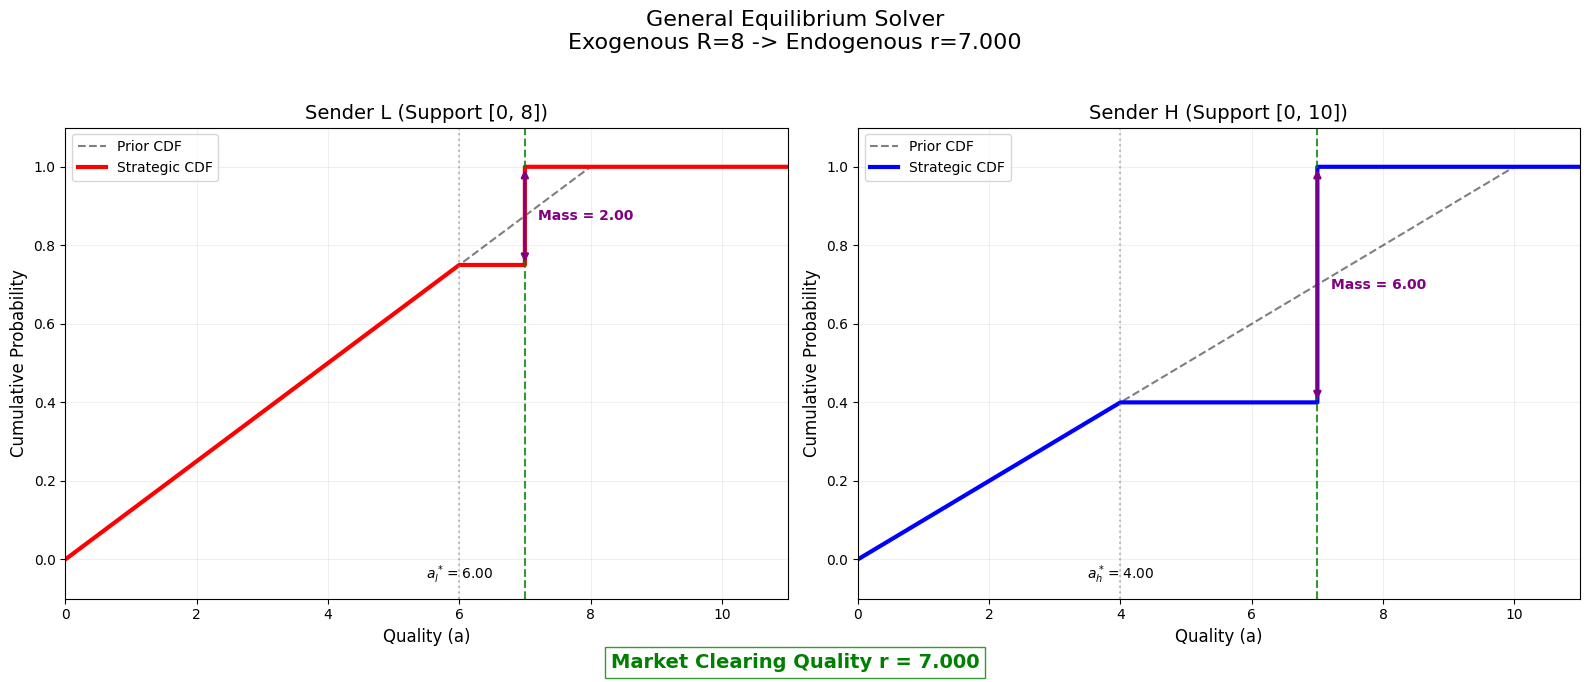
\includegraphics[width=1\linewidth]{Example 1.png}
    \caption{Uniform Distribution of Products}
    \label{fig:example1}
\end{figure}

In equilibrium, we have $r=7$, $a^*_l=6$ and $a^*_h=4$. It turns out that $l$ places two products with quality $6\leq a\leq 8$ and $h$ places six with quality $4\leq a \leq 10$. However, under perfect sorting when products are sorted by the actual $a$, sender $h$ should only place two more products. Inefficiency arises as some worse products are selected while the better are dismissed. It is also detrimental to equity when products are people (e.g. students). 

Abstract away from real numbers. Let $F_h(a)=a$ for $a \leq \bar{a}_h$ and $F_l(a)=a$ for $a \leq \bar{a}_l$, and assume $q_h/q_l=\bar{a}_h/\bar{a}_l$. One can easily show that given any $R$, sender $h$ places $(2a_h-2r)$ products and sender l places $(2a_l-2r)$. The difference in the number of products placed is twice the difference in their maximum qualities. Therefore, sender $h$ can always gain an unfair advantage from a better distributed $F_h(\cdot)$, strategically placing more products than in the perfect sorting case. 


\subsection{Advantaged Sender}

Sometimes at given $R$, we do not have the prior problem about inefficiency, and products are placed if and only if it has actual quality $a\geq a^*$, no matter which sender it belongs to \footnote{When $R$ is large such that sender $h$ places all products, we don't have the inefficiency problem although $a^*_l <a^*_h$. However, we only look at interior solutions}. We name it perfect separation.

\begin{definition}
    \label{def: Perfect Separation}
    We have perfect separation at $r$ if in equilibrium we have $a^*_h=a^*_l=a^*$ with corresponded $R$. 
\end{definition}

To formally check whether perfect separation occurs, recall:
\[
        r =\mu_i(a_i^*)= \mathbb{E}_{F(\cdot)}[a \mid a \geq a^*_i]
    \]
Since $a^*_i$ is continuous and $\mu_i(\cdot)$ is strictly increasing, the reverse function is also continuous and strictly increasing in $r$:
\[
        a_i^*=\mu^{-1}_i(r)
    \]
In equilibrium $r$ is determined. Difference in the minimum quality of products placed between two senders is:
\[d(r)=\mu_l^{-1}(r)-\mu_h^{-1}(r)\]

Therefore, another way to say Definition \ref{def: Perfect Separation} is that we have perfect separation at $r$ if and only if $d(r)=0$. 

Now, we give a formal definition of being "advantaged". We say one distribution $n_h^*(\cdot)$ is advantaged relative to $n_l^*(\cdot)$ if at any common support $a^*_i$, $\mu_h(a_i^*)>\mu_l(a_i^*)$.

\begin{definition}
    \label{def: advantaged}
    Consider two distributions with cumulative distribution functions (CDFs) $n_h^*$ and $n_l^*$, supported on $[\underline{a}_h, \bar{a}_h]$ and $[\underline{a}_l, \bar{a}_l]$ respectively. We say that $n_h^*$ is \textbf{advantaged} over $n_l^*$ if for all $a^*_i$ in the common support:\[
        \mu_h(a^*_i) > \mu_l(a^*_i)
    \]Intuitively, this implies that $n_h^*$ strictly dominates $n_l^*$ in terms of mean residual life wherever interior solution of $a^*_l$ and $a^*_h$ exists.
\end{definition}


\subsection{Baseline Incompatibility}

We can formalize the prior matching inefficiency through a classical mechanism design lens. Let the state variable be $\theta = (n_h^*(\cdot), n_l^*(\cdot), R) \in \Theta$, which encapsulates the broad state space of all possible continuous true quality distributions for both senders and any exogenous capacity limit. Denote $L$ as the summation of the true expected qualities of the products that are selected to fill the capacity $R$. The Social Planner aims at maximizing $\alpha \cdot L$. Given the continuous distributions, we define the Social Choice Function (SCF), $\phi(\theta)$, as the mapping to an optimal allocation where all products with a real quality higher than a unified threshold $a^{eff}$ are selected. 

Why doesn't the social planner directly intervene, mandating each sender to place this socially optimal quantity? In our setting, the planner does not have direct dictatorial control over the placement. Instead, small, decentralized receivers with no market power independently decide whom to accept based on pooled expected quality, which endogenously clears $R$. Thus, we must evaluate if the baseline game naturally implements the SCF.

\begin{theorem}[Necessary Condition for Efficient Realization]
\label{Theorem: Impossibility of Baseline}
    Consider an interior baseline equilibrium. If the baseline subgame without intervention implements the aligned social choice rule $\phi(\theta)$, then the state $\theta$ must strictly satisfy:
    \[
        \mu_h(a^{eff}) = \mu_l(a^{eff})
    \]
    Therefore, under any state $\theta$ for which $\mu_h(a^{eff}) \neq \mu_l(a^{eff})$, the equilibrium from baseline game doesn't meet $\phi(\theta)$. Intuitively, the equality generically fail, and $\phi(\cdot)$ cannot be implemented if receivers sort by expected qualities. 
\end{theorem}

\begin{proof}
    Suppose there exists an interior baseline equilibrium $NE(\theta)$ that successfully implements the social choice function $F$. By definition of $\phi (\theta)$, the endogenous subgame cutoffs must perfectly align at the efficient threshold: $a_h^* = a_l^* = a^{eff}$.
    
    In any interior baseline equilibrium, receivers independently select products based on expected quality, which systematically forces the market standard to clear at a uniform expected quality $r_0$. Thus, the equilibrium strictly requires the conditional expectations of the placed products to be equal:
    \[
        r_0 = \mu_h(a_h^*) = \mu_l(a_l^*)
    \]
    Substituting the SCF requirement $a_h^* = a_l^* = a^{eff}$ into this necessary equilibrium condition yields:
    \[
        \mu_h(a^{eff}) = \mu_l(a^{eff})
    \]
    This proves that the coincidence of the conditional expectations at the threshold $a^{eff}$ is a strict prerequisite for the baseline game to yield the efficient allocation. Consequently, if the state $\theta$ is such that $\mu_h(a^{eff}) \neq \mu_l(a^{eff})$, no interior equilibrium can achieve $a_h^* = a_l^* = a^{eff}$, meaning the baseline game inherently fails to implement $\phi (\theta)$.
\end{proof}

Economically, the necessary condition $\mu_h(a^{eff}) = \mu_l(a^{eff})$ is a highly fragile, knife-edge requirement. It demands that two distinctly independent quality distributions yield the exact same conditional expected quality at a specific capacity-clearing threshold. Because this singular equality is generally non-robust to minor perturbations in the underlying distributions $F_i(\cdot)$ or the capacity $R$, the baseline uniform market is pervasively incompatible with the efficient allocation rule. This structural failure necessitates external intervention via a mechanism design approach.

\begin{corollary}
If sender $h$ is advantaged over sender $l$ in the sense of Definition \ref{def: advantaged}, then no interior baseline equilibrium can implement $\phi (\theta)$.
\end{corollary}

\section{Prize Scheme}

\subsection{Setup}
We introduce a piece-wise reward scheme $(r_2, A_2)$ to relieve the mismatch: In addition to the base prize $A_1$ for securing a standard placement (at expected quality $r_1$), an extra prize $A_2$ is awarded to products reaching a higher expected quality $r_2$. We assume $r_2$ is larger than initial $r_1$ with no prize scheme (denoted as $r_0$). Senders now face a trade-off: separating top candidates captures the premium $A_2$, but it extracts high-quality products from their distribution, reducing their advantage in the subsequent competition for $A_1$.

To formalize this, consider sender $i$ with an original probability density function $f_i^*(a)$ and maximum quality $\bar{a}_i$. To form the premium pool, sender $i$ does not need to extract a continuous upper-tail interval; instead, they can selectively pool products to exactly match the target $r_2$. To form the premium pool, sender $i$ chooses an extraction density $w_i(a)$ over the quality support $[\underline{a}_i,\bar{a}_i]$, subject to a mass constraint and a mean constraint with target $r_2$. 


Sender $i$'s optimal separation strategy is characterized by a weight function $w_i(a)$, representing the density of products allocated to the premium pool. Let $W_i = \int_{\underline{a}_i}^{\bar{a}_i} w_i(a) \, \mathrm{d}a$ denote the total mass of the separated products. By extracting $w_i(\cdot)$, sender $i$ is left with a depleted distribution for the standard Subgame, characterized by the new density of product:
$$ \tilde{f}_i(a) =f_i^*(a) - w_i(a) $$
Let $\tilde{n}_i(\cdot)$ denote the corresponding modified CDF of these remaining products. 

After extracting $w_i(\cdot)$, senders are playing in a subgame. Let $Q_i(w_i,w_{-i})$ be the total mass of products sender $i$ successfully places in the subgame (earning only $A_1$) when playing with $w_i$ with depleted distribution $\tilde{n}_i$ against the competitor's strategy $w_{-i}(\cdot)$. We can then formalize the Best Correspondence of Senders. In equilibrium, sender $i$ choose an optimal $w^*_i(\cdot)$ which maximize the summation of rewards from the subgame and $W^*_i$:
$$ U_i:=W^*_i (A_1 + A_2) + A_1 \cdot Q_i(w^*_i(\cdot),w^*_{-i}(\cdot)) $$

Subject to the constraints:
$$ 0 \leq w_i(a) \leq f_i^*(a) \quad \forall a \in [\underline{a}_i, \bar{a}_i] $$
$$ \int_{\underline{a}_i}^{\bar{a}_i} (a - r_2) w_i(a) \, \mathrm{d}a = 0 $$
\subsection{Simplify the Problem}

At first glance, sender $i$'s strategy space is highly complex: they must choose a functional shape $w_i(x)$ for the premium pool, while considering how this extraction dynamically alters the endogenously determined subgame market-clearing quality $r_1$ and their own subgame cutoff $a_{1,i}^*$. 

Extracting products for the premium pool imposes a "quality burden" on the sender's subgame performance, as they lose high-quality products that could have been used to disguise lower-quality ones. We define this quality burden $K_i$, which is a function of the cutoff $a_{1,i}^*$ and market standard $r_1$, as the extracted quality slack above the cutoff:
\[
    K_i(a_{1,i}^*, r_1) \equiv \int_{a_{1,i}^*}^{\bar{a}_i} (x - r_1) w_i(x) \, \mathrm{d}x 
\]

The following lemmas drastically simplify the sender's functional optimization problem, proving that certain extraction behaviors are strictly dominated in the general equilibrium.

\textbf{Remark 1 (Market Standard Depreciation).} 
Before proceeding to the sender's optimal extraction strategy, we must clarify the fundamental relationship between the premium target $r_2$, the original market standard $r_0$, and the endogenous subgame standard $r_1$. By mechanism design, the premium target is strictly higher than the original uniform standard ($r_2 > r_0$). When an advantaged sender extracts top-tier products to capture the premium prize $A_2$, their remaining distribution in the standard subgame is systematically depleted of its highest qualities (a "brain drain" effect). Because the total exogenous capacity $R$ must still be cleared, the market must compensate for this loss of high-quality supply by lowering the clearing threshold. Consequently, the new subgame standard $r_1$ is strictly driven below the original standard ($r_1 < r_0$). This intrinsic market adjustment mathematically guarantees the strict ordering $r_2 > r_0 > r_1$, ensuring that the premium pool unequivocally represents a strictly higher quality standard than the residual subgame.

\begin{lemma}[No Downward Cherry-Picking]
\label{Lemma: No Cherry Picking}
In equilibrium, sender $i$ will never extract products with qualities below their subgame cutoff $a_{1,i}^*$ to form the premium pool. That is, $w_i(x) = 0$ for all $x < a_{1,i}^*$. 
\end{lemma}

Eliminating this downward cherry-picking yields a striking property regarding the shape of $w_i(x)$.

\begin{lemma}[Shape Independence]
\label{Lemma: Shape Independence}
Given Lemma \ref{Lemma: No Cherry Picking}, the penalty imposed on the subgame depends exclusively on the total extracted mass $W_i$. Specifically, $K_i(a_{1,i}^*, r_1) \equiv (r_2 - r_1)W_i$. Consequently, the specific functional shape of the extraction $w_i(x)$ above the cutoff has no impact on the subgame equilibrium. 
\end{lemma}

These two lemmas act as a dimensional reduction for our mechanism design problem. Because the subgame equilibrium is completely immune to the functional shape of $w_i(x)$ and responds only to the scalar volume $W_i$, the Social Planner does not need to worry about complex functional deviations from the senders. 

\subsection{Equilibrium}

To understand the senders' equilibrium strategies, we first formalize their objective function and define the marginal cost of separating products into the premium pool. 

Suppose the standard placement in the subgame rewards $A_1$, and the premium pool offers an additional $A_2$ (yielding $A_1 + A_2$ in total). Let $Q_i$ denote the mass of products sender $i$ successfully places in the subgame. Since sender $i$ extracts $W_i$ from their total distribution, $Q_i$ is determined by the endogenous subgame cutoff $a_{1,i}^*$:
$$Q_i = \int_{a_{1,i}^*}^{\bar{a}_i} f_i^*(x) \, \mathrm{d}x - W_i$$

Sender $i$'s total payoff $\Pi_i$ is the sum of rewards from both pools:
$$\Pi_i = W_i(A_1 + A_2) + Q_i A_1 = W_i A_2 + A_1 \int_{a_{1,i}^*}^{\bar{a}_i} f_i^*(x) \, \mathrm{d}x$$
Recall the maximum $W_i$ senders can choose are restricted by capacity constraints: 
\[W_i \leq \int_{a^*_{2,i}}^{\bar{a}_i}f^*(x)\cdot dx=\bar{W}_i\]
Define $a^*_{2,i}$ as another threshold:
\[r_2=\mathbb{E}_{f^*(\cdot)}[a \mid a \geq a^*_{2,i}]\]

Taking the partial derivative of the payoff with respect to $W_i$ yields the marginal net benefit of extraction:
$$\frac{\partial \Pi_i}{\partial W_i} = A_2 - A_1 \left( f_i^*(a_{1,i}^*) \frac{\partial a_{1,i}^*}{\partial W_i} \right)$$

The term in the parentheses represents the marginal density of products lost in the subgame due to the forced increase in the placement cutoff $a_{1,i}^*$. We define this as the "Marginal Cost of Separation", denoted as $MC_i \equiv f_i^*(a_{1,i}^*) \frac{\partial a_{1,i}^*}{\partial W_i}$. For a sender to have an incentive to separate products, the prize ratio must exceed this marginal cost ($\frac{A_2}{A_1} > MC_i$). We define the prize ratio as $\tau$. It's easy to observe that only the ratio matters. 

The following lemma analytically characterizes this marginal cost and reveals a crucial asymmetry between the two senders.

\begin{lemma}[Marginal Cost of Separation]
\label{Lemma: Marginal Cost}
Given the general equilibrium of the subgame, if the marginal cost is defined ($\bar{W}_i > 0$), the marginal cost of extraction $MC_i$ for sender $i \in \{h, l\}$ is strictly non-negative and is globally characterized by:
$$MC_i = \frac{(r_2 - r_1)Q_{-i}}{Q_{-i}(r_1 - a_{1,i}^*) + Q_i(r_1 - a_{1,-i}^*)}$$
Consequently, if the competitor completely exhausts their capacity in the subgame ($Q_{-i}=0$), the marginal cost inherently drops to zero ($MC_i=0$). Furthermore, in any interior subgame equilibrium where both senders maintain active placements ($Q_h, Q_l > 0$), the marginal costs are strictly positive, and their ratio is inversely proportional to their respective placement quantities:
$$\frac{MC_h}{MC_l} = \frac{Q_l}{Q_h}$$
\end{lemma}

The proof is provided in the Appendix. Lemma \ref{Lemma: Marginal Cost} captures the soul of the piece-wise prize mechanism. In the original inefficient market, the advantaged sender $h$ dominates the placement capacity. The inverse proportionality dictates that $MC_h \ll MC_l$. The sender who occupies more subgame capacity inherently faces a lower marginal cost to separate high-quality products. 

Therefore, by carefully setting the prize ratio $\tau$ between $MC_h$ and $MC_l$, the social planner can induce a unilateral separation where only the advantaged sender extracts top products. Since $MC_i$ is strictly positive, $a^*_{1,i}$ is strictly increasing in $W_i$. Therefore, choosing prize ratio in that way is sufficient to increase placement from disadvantaged sender and improve matching efficiency. We are now interested in specific range of $\tau$ such that the benefit is maintained. In fact, we proved that the range of it is highly robust.  

Before evaluating the effects of the piece-wise prize scheme, we must formally define the capacity constraints of the senders. Let $S_i(a) =q_i \cdot (1-F(a))$ denote the survival function, representing the total mass of products with quality above threshold $a$. 

Consider the original equilibrium without the piece-wise prize, where the market clearing standard is $r_0$. The total mass of products placed by sender $i$ is $P_i^0 = S_i(a_i^0)$, where $a_i^0$ satisfies $\mu_i(a_i^0) = r_0$. 

When the piece-wise prize $A_2$ is introduced with a target expected quality $r_2$ ($r_2 > r_0$), the absolute maximum mass of premium products sender $i$ can physically extract from its distribution is denoted as $\bar{W}_i$. This maximum capacity is achieved by extracting all products above a threshold $a_{2,i}^*$ such that the expected quality exactly equals $r_2$. Therefore, $\bar{W}_i = S_i(a_{2,i}^*)$, where $\mu_i(a_{2,i}^*) = r_2$.

The ratio $\bar{W}_i / P_i^0$ represents the conditional probability that a product qualifies for the premium pool, given that it was already qualified for the standard pool in the original equilibrium. The following Lemma proves that the "advantaged" property defined in Definition \ref{def: advantaged} inherently guarantees a strictly fatter upper tail in this relative proportion.

\begin{lemma}[Proportional Premium Capacity]
\label{Lemma: Proportional Premium Capacity}
If sender $h$ is advantaged over sender $l$ (i.e., $\mu_h(a) > \mu_l(a)$ in the common support), then sender $h$ inherently possesses a fatter upper tail in its distribution of product qualities, such that:
\[
    \frac{\bar{W}_h}{P^0_h} > \frac{\bar{W}_l}{P^0_l}
\]
\end{lemma}

Using Lemma \ref{Lemma: Proportional Premium Capacity}, we demonstrate that as long as sender $h$ is advantaged and initially places more products, introducing the piece-wise prize scheme strictly shifts market placement from sender $h$ to sender $l$. Intuitively, to capture the premium prize $A_2$, sender $h$ is incentivized to extract a disproportionately larger share of its high-quality products, thereby eroding its competitive advantage in the subsequent subgame. Formally, we show that when $P^0_h \geq P^0_l$, any active equilibrium must fall into one of four distinct regimes: (1) an interior equalized subgame ($Q_l=Q_h$, with $W_i \leq \bar{W}_i$), (2) unilateral separation by the advantaged sender ($W_l=0$, $\bar{W_l}>0$, $W_h > 0$), (3) capacity exhaustion by the advantaged sender ($W_l > 0$, $W_h=\bar{W}_h$), or (4) no capability for disadvantaged sender ($\bar{W_l}=0, W_h > 0$). The rigorous derivation of these states is embedded in the proof of Lemma \ref{Lemma: Placement Shift}.

\begin{lemma}[Placement Shift]
\label{Lemma: Placement Shift}
    If sender $h$ is advantaged over sender $l$ and places more products in the original game, the introduction of a piece-wise prize scheme $(r_2, A_2)$ will strictly decrease the total product placement from the advantaged sender $h$ and strictly increase the placement from the disadvantaged sender $l$ if and only if the prize ratio is sufficiently high to activate separation, i.e., $\tau > MC^0_h$, where $MC_i^0$ evaluates the marginal cost of separation at the original uniform equilibrium.
\end{lemma}

However, if sender $h$ places fewer products in the original game due to a smaller total mass $q_h$, the mechanism faces a unique challenge. The following Lemma establishes the exact boundary conditions for a placement shift when $P_h^0 \le P_l^0$, revealing that conventional interior prize schemes completely fail.

\begin{lemma}[Placement Shift under Initial Minority]
\label{Lemma: Boutique Advantaged Sender}
    Assume sender $h$ is advantaged over sender $l$, but places no more products in the original uniform game ($P_h^0 \le P_l^0$). 
    1. \textbf{Impossibility of Interior Shift:} Any piece-wise prize scheme $(r_2, A_2)$ that results in an interior equilibrium (where neither sender exhausts their premium capacity, $W_i^* < \bar{W}_i$) will strictly fail to produce a placement shift, and will instead exacerbate the mismatch ($P_h^* \ge P_h^0$).
    2. \textbf{Sufficiency of Corner Solutions:} The Social Planner can only successfully induce a placement shift ($P_h^* < P_h^0$ and $P_l^* > P_l^0$) by utilizing extreme mechanisms that drive the disadvantaged sender to a corner solution. Specifically, a shift is guaranteed if:
        a) \textit{Exclusive Premium:} Assuming the prize ratio is sufficient to activate the mechanism ($\tau > MC_h^0$), the target is set above the disadvantaged sender's physical limit ($r_2 \ge \bar{a}_l$), forcing $\bar{W}_l = 0$.
        b) \textit{Mutual Exhaustion:} The prize $A_2$ is set astronomically high such that both senders exhaust their premium capacities ($W_i^* = \bar{W}_i$).
\end{lemma}

Lemma \ref{Lemma: Boutique Advantaged Sender} provides a profound implication for Mechanism Design. When dealing with a "boutique" advantaged sender, marginal incentive alignment is impossible. The Social Planner must resort to corner solutions---either cornering the target quality to physically exclude the disadvantaged sender, or cornering the prize magnitude to exhaust all available capacities.


\subsection{Conditions to Improve Efficiency}

In the previous section, we established that the introduced prize scheme can successfully induce a placement shift from the advantaged sender to the disadvantaged. Usually, this shift strictly reduces the discrepancy between the subgame cutoffs $a^*_{1, h}$ and $a^*_{1, l}$. However, if the placement shift is too aggressive, it can cause $a^*_{1, h} > a^*_{1, l}$ in equilibrium, introducing a new inefficiency where mediocre products from sender $l$ crowd out superior products from sender $h$ (overshooting). 

Our ultimate aim is to make the matching inefficiency $|a^*_{1, l}-a^*_{1, h}|$ as small as possible, ideally zero. To clearly illustrate how the Social Planner can perfectly calibrate this mechanism, we focus on the case where the advantaged sender initially dominates the market ($P_h^0 > P_l^0$), and we break down the necessary conditions to achieve optimal efficiency step by step.

\textbf{Step 1: Defining the Target State}

To define the boundary of an optimal correction, we define the \textbf{Perfect Alignment} state where the mechanism successfully equalizes the subgame cutoffs without overshooting, i.e., $a^*_{1,h} = a^*_{1,l} = a^{eff}$. 
Recall that total placement is $Q_i + W_i = S_i(a_{1,i}^*)$, where $S_i(\cdot)$ is the exogenous survival function (adjusted for $q$). The global market clearance strictly requires $S_h(a_{1,h}^*) + S_l(a_{1,l}^*) = R$. Therefore, the perfect alignment target cutoff $a^{eff}$ is a unique, fixed constant entirely determined by the exogenous capacity constraint: $S_h(a^{eff}) + S_l(a^{eff}) = R$.

\textbf{Step 2: Identifying the Required Physical Extraction}

To clearly isolate the marginal incentives from physical capacity constraints, we must determine how much the advantaged sender needs to extract to reach this ideal state. Assuming a purely unilateral shift where the disadvantaged sender does not extract ($W_l = 0$), let $\hat{W}_h$ denote the exact theoretical mass sender $h$ must separate into the premium pool to achieve this perfect alignment state. From the subgame quantity definition, this required extraction is explicitly determined by $\hat{W}_h = S_h(a^{eff}) - Q_h^{eff}$.

\begin{lemma}[Strict Positivity of Target Extraction]
\label{Lemma: Positive Target Extraction}
If sender $h$ is advantaged over sender $l$, the theoretical mass $\hat{W}_h$ required to achieve the perfect alignment state ($a_{1,h}^* = a_{1,l}^* = a^{eff}$) via unilateral separation is strictly positive ($\hat{W}_h > 0$).
\end{lemma}

This fundamental property guarantees that driving the system toward optimal efficiency strictly requires the advantaged sender to pay a real cost, ensuring the equilibrium marginal cost strictly increases ($MC_h^{eff} > MC_h^0$).


\textbf{Step 3: The Incentive Condition for Unilateral Separation}

To ensure that the Social Planner can achieve this unilateral alignment without accidentally triggering extraction from the disadvantaged sender $l$, the advantaged sender must possess a sufficiently fat upper tail at this specific target coordinate to maintain subgame dominance. We formalize this structural requirement using the Quality Deficit Integral: $D_i(a) = \int_a^{\bar{a}_i} (r_2 - x) f_i^*(x) \, \mathrm{d}x$.

The following lemma establishes a powerful linear relationship between this integral and the subgame placement quantity.

\begin{lemma}[Equivalence of Quality Deficit and Subgame Quantity]
\label{Lemma: Quantity Equivalence}
    In any subgame equilibrium, the total mass of products sender $i$ places in the standard pool ($Q_i$) is strictly proportional to their Quality Deficit Integral $D_i(a_{1,i}^*) = \int_{a_{1,i}^*}^{\bar{a}_i} (r_2 - x) f_i^*(x) \, \mathrm{d}x$. Specifically:
    \[
        (r_2 - r_1)Q_i = D_i(a_{1,i}^*)
    \]
    Consequently, at the perfect alignment state ($a_{1,h}^* = a_{1,l}^* = a^{eff}$), sender $h$ maintains quantity dominance in the subgame ($Q_h^{eff} \ge Q_l^{eff}$) if and only if $D_h(a^{eff}) \ge D_l(a^{eff})$.
\end{lemma}

\begin{proof}
    Recall the definition of the subgame quantity $Q_i = S_i(a_{1,i}^*) - W_i$. 
    From the subgame equilibrium condition, we have:
    \[
        \int_{a_{1,i}^*}^{\bar{a}_i} (x - r_1) f_i^*(x) \, \mathrm{d}x = (r_2 - r_1)W_i
    \]
    We can rewrite the term $(x - r_1)$ in the integrand as $-(r_2 - x) + (r_2 - r_1)$:
    \[
        -\int_{a_{1,i}^*}^{\bar{a}_i} (r_2 - x) f_i^*(x) \, \mathrm{d}x + \int_{a_{1,i}^*}^{\bar{a}_i} (r_2 - r_1) f_i^*(x) \, \mathrm{d}x = (r_2 - r_1)W_i
    \]
    Substituting the definition of the Quality Deficit Integral $D_i(a_{1,i}^*)$ and the survival function $S_i(a_{1,i}^*)$ yields:
    \[
        -D_i(a_{1,i}^*) + (r_2 - r_1)S_i(a_{1,i}^*) = (r_2 - r_1)W_i
    \]
    Rearranging the terms, we elegantly factor out $(r_2 - r_1)$:
    \[
        D_i(a_{1,i}^*) = (r_2 - r_1)(S_i(a_{1,i}^*) - W_i) = (r_2 - r_1)Q_i
    \]
    Because $r_2 > r_1$ in any active mechanism, $Q_i$ and $D_i(a_{1,i}^*)$ are strictly proportional. Therefore, evaluating this relation at the common perfect alignment cutoff $a^{eff}$ with a common standard $r_1$ yields the strict equivalence: $Q_h^{eff} \ge Q_l^{eff} \iff D_h(a^{eff}) \ge D_l(a^{eff})$.
\end{proof}

By Lemma \ref{Lemma: Quantity Equivalence}, we can now mathematically formalize the structural prerequisite for efficiency improvement:

\begin{assumption}
\label{As: Strong Advantage Condition}
    \textbf{Strong Advantage Condition:} At the fixed target $a^{eff}$, the advantaged sender must maintain a larger quality deficit integral: $D_h(a^{eff}) \ge D_l(a^{eff})$. This guarantees that even when perfect alignment is reached, the advantaged sender naturally maintains a larger placement share ($Q_h^{eff} \ge Q_l^{eff}$).
\end{assumption}


\textbf{Step 4: Ensuring Mathematical Stability (Well-Behaved Payoffs)}

Finally, to guarantee that the senders' extraction decisions converge to a predictable, unique, and stable interior point without boundary erraticism, we must impose a standard regularity condition on their objective functions.

\begin{assumption}[Well-Behaved Payoffs]
    \label{As: Regularity of Survival Function}
    We assume the marginal cost of extraction $MC_i(W_i, W_{-i})$ is continuously differentiable and strictly monotonically increasing with a strictly positive partial derivative with respect to its own extraction $W_i$, given $W_{-i}$ unchanged ($\frac{\partial MC_i}{\partial W_i} > 0$). Equivalently, this ensures that each sender's objective function $\Pi_i(W_i, W_{-i})$ is globally strictly concave in their own extraction. 
\end{assumption}

This assumption is not difficult to satisfy. One explicit mathematical sufficient condition for this regularity is as follows:

\begin{lemma}[Sufficient Condition for Strict Convexity]
    \label{Lemma: Sufficient Condition for Convexity}
    Assume the baseline distributions are continuously differentiable. On the unilateral extraction locus ($W_l = 0$), Assumption \ref{As: Regularity of Survival Function} holds if the disadvantaged sender's distribution $f_l^*(\cdot)$ globally satisfies the Weak Mean-to-Hazard Bound (MHB):
    \[
        \mu_l(a) - a \ge \frac{1}{2} \frac{S_l(a)}{f_l^*(a)}
    \]
    where $\mu_l(a) = \mathbb{E}[x \mid x \ge a]$ is the conditional expectation, and $S_l(a) / f_l^*(a)$ is the inverse hazard rate. 
\end{lemma}

This is a purely exogenous shape condition on the probability distribution. It simply requires that the conditional expected quality ($\mu_l$) is not pathologically close to the cutoff ($a$). For example, a Uniform distribution yields exactly $\mu(a) - a = \frac{1}{2}\frac{S(a)}{f(a)}$ (satisfying it with equality), while an Exponential distribution yields $\mu(a) - a = \frac{S(a)}{f(a)}$ (satisfying it strictly). Thus, regular distributions naturally guarantee the convexity of the mechanism.

\textbf{Step 5: Synthesizing the Efficiency Improvement}

With the target defined, the incentive structure validated, and the mathematical stability secured, we can now formally establish the boundaries within which the Social Planner can successfully improve matching efficiency.

\begin{proposition}[Sufficient Condition for Efficiency Improvement]
    \label{prop: Efficiency Improvement}
    Under Assumption \ref{As: Regularity of Survival Function}, suppose $D_h(a^{eff}) > D_l(a^{eff})$, sender $h$ has adequate premium physical capacity ($\bar{W}_h \geq \hat{W}_h$), and in the original equilibrium $P_h^0 > P_l^0$. 
    
    If the prize ratio satisfies
    $$MC_h^0 < \tau \leq MC_h^{eff},$$
    then there exists a unique equilibrium on the unilateral branch with $W_l^* = 0$ and $W_h^* \in (0, \hat{W}_h]$. This equilibrium is strict, hence locally stable under best-response dynamics. Its cutoffs satisfy
    $$a_h^0 < a_h^* \leq a^{eff} \leq a_l^* < a_l^0.$$
    The middle equalities hold if and only if $\tau = MC_h^{eff}$; equivalently, if $MC_h^0 < \tau < MC_h^{eff}$, then
    $$a_h^0 < a_h^* < a^{eff} < a_l^* < a_l^0.$$
    Consequently, the matching inefficiency $|a_h^* - a_l^*|$ is strictly smaller than the original $|a_h^0 - a_l^0|$, and no overshooting occurs ($a_h^* \leq a_l^*$).
\end{proposition}

Note that the strict monotonicity of $MC_h$ combined with $\hat{W}_h > 0$ mathematically guarantees that the interval $(MC_h^0, MC_h^{eff}]$ is non-empty.


\subsection{Conditions to Improve Equality}

Preserve assumptions in last subsection, we can easily find conditions to improve equality.

\begin{proposition}[Exogenous Sufficient Condition for Equality Improvement]
\label{prop:SC_equality}
Assume the mechanism induces an efficiency-improving unilateral separation ($W_l^*=0$), and the marginal cost $MC_h(W_h,0)$ is strictly increasing in $W_h$. If the prize ratio satisfies:
\[
MC_h^0 < \tau \le \frac{R}{P_l^0} MC_h^0
\]
then there exists a unique equilibrium in which mechanism strictly improves equity, i.e.,
\[
\frac{U_l^*}{U_h^*} > \frac{U_l^0}{U_h^0}
\]
\end{proposition}

Therefore, if the social planner set $MC_h^0 < \tau \le \min(\frac{R}{P_l^0} MC_h^0,MC_h^{eff})$, there is a free lunch: both equality and matching efficiency is improved by the introduction of prize scheme. We have proved that such $\tau$ always exists under Assumption \ref{As: Strong Advantage Condition} and Assumption \ref{As: Regularity of Survival Function}.


\section{Social Planner Problem}

\subsection{Decentralizing the Social Choice Function}

In Section \ref{sec: Subgame Equilibrium}, we established via Theorem \ref{Theorem: Impossibility of Baseline} that the Social Choice Function $\phi (\theta)$, which achieves perfect matching alignment ($a_h = a_l = a^{eff}$), cannot be implemented in the baseline game because receivers independently make decentralized decisions based on pooled expected qualities.

We now prove that if the Social Planner can observe the true state $\theta$ (the quality distributions $F_i(\cdot)$ and capacity $R$), they can design a piece-wise prize scheme $M = (r_2, \tau)$ to successfully decentralize $\phi (\theta)$. That is, the planner can calibrate the prize scheme such that the socially optimal allocation emerges as a unique, locally stable unilateral-separation equilibrium.

\begin{theorem}[Decentralization via Piece-Wise Prize]
\label{Theorem: Implementation}
    Assume the Social Planner observes the true state $\theta$. Fix a premium target $r_2$ such that the strict deficit condition
    \[
        D_h(a^{eff}) > D_l(a^{eff})
    \]
    holds. Suppose further that the baseline conditions $P_h^0 > P_l^0$ and physical premium slack ($\bar{W}_h \geq \hat{W}_h$) hold, and that Assumption \ref{As: Regularity of Survival Function} is satisfied. 
    
    The Social Planner can decentralize the social choice function $\phi (\theta)$ by setting a piece-wise prize scheme $M = (r_2, \tau^*)$ where $\tau^* = MC_h^{eff}$. Under this mechanism, there exists a unique strict equilibrium on the unilateral branch, hence a unique locally stable unilateral-separation equilibrium, and it satisfies
    \[
        (W_h^*, W_l^*) = (\hat{W}_h, 0)
        \quad \text{and} \quad
        a_{1,h}^* = a_{1,l}^* = a^{eff}.
    \]
\end{theorem}

\begin{proof}
    Set $\tau^* = MC_h^{eff}$. The assumptions of Proposition \ref{prop: Efficiency Improvement} are then satisfied for the chosen $r_2$. Therefore the induced game has a unique equilibrium on the unilateral branch with $W_l^* = 0$ and $W_h^* \in (0,\hat{W}_h]$. This equilibrium is strict, hence locally stable, and its cutoffs satisfy
    \[
        a_h^0 < a_{1,h}^* \le a^{eff} \le a_{1,l}^* < a_l^0.
    \]
    Because $\tau^* = MC_h^{eff}$, Proposition \ref{prop: Efficiency Improvement} further gives the middle equalities, so
    \[
        a_{1,h}^* = a_{1,l}^* = a^{eff}.
    \]
    Since $MC_h(\cdot,0)$ is strictly increasing and $MC_h(\hat{W}_h,0)=MC_h^{eff}=\tau^*$, the unique solution on the unilateral branch is $W_h^*=\hat{W}_h$.

    It remains to verify that the implemented allocation coincides with $\phi(\theta)$. Because $W_l^*=0$ and both standard-pool cutoffs equal $a^{eff}$, the standard pool contains exactly the mass of products with quality at least $a^{eff}$ that are not extracted. By Lemma \ref{Lemma: No Cherry Picking}, the premium pool extracted by sender $h$ also contains only products with quality at least $a^{eff}$. Hence every selected product under the mechanism has true quality at least $a^{eff}$. Total selected mass is
    \[
        S_h(a^{eff}) + S_l(a^{eff}) = R,
    \]
    so the mechanism selects exactly the capacity-filling set of products above the efficient cutoff. This is precisely $\phi(\theta)$.
\end{proof}


\subsection{Dynamic Convergence with Unobservable Quality}

In Theorem \ref{Theorem: Implementation}, we established that the Social Planner can decentralize the Social Choice Function if they observe the true state $\theta$ ex-ante to analytically compute exactly $\tau^* = MC_h^{eff}$. In many realistic policy environments, however, the underlying true quality distributions $F(\cdot)$ are private or unobservable ex-ante. 

To bridge this informational gap, we model a dynamic learning mechanism where the planner adjusts the piece-wise prize scheme over discrete periods $t = 1, 2, \dots$. While the true distribution is unobservable beforehand, we introduce a standard and highly practical ex-post observability assumption.

\begin{assumption}[Delayed Observation of Marginal Quality]
\label{As: Delayed Observation}
    While the planner cannot observe the full true quality distributions $F^*(\cdot)$, they can observe the realized true quality of the marginal products successfully placed in the standard pool (i.e., the actual subgame cutoffs $a_{1,h}^{*(t)}$ and $a_{1,l}^{*(t)}$) with a one-period delay, after the market clears.
\end{assumption}

Economically, this maps to scenarios where receivers (e.g., universities or employers) accept candidates based on disguised expected qualities, but the planner (e.g., the government) can subsequently audit and measure the actual true performance of the marginally accepted candidates in the following period.

With this delayed feedback, the planner can utilize a simple, gradient-based Tâtonnement updating rule to iteratively discover the optimal prize ratio $\tau^*$. We define the observable matching mismatch error in period $t$ as $\Delta^{(t)} = a_{1,l}^{*(t)} - a_{1,h}^{*(t)}$. 

\begin{theorem}[Local Dynamic Convergence]
\label{Theorem: Dynamic Convergence}
    Assume all static prerequisites for decentralization hold (i.e., $P_h^0 > P_l^0$, physical premium slack $\bar{W}_h > \hat{W}_h$, the Strict Strong Advantage Condition, and Assumption \ref{As: Regularity of Survival Function}). 
    
    Consider the dynamic updating rule:
    \[
        \tau^{(t+1)} = \tau^{(t)} + \gamma \cdot \Delta^{(t)}
    \]
    There exists a neighborhood $U$ around the optimal prize ratio $\tau^*$ and a threshold $\bar{\gamma} > 0$ such that for any initial active prize ratio $\tau^{(1)} \in U$ and any learning rate $\gamma \in (0, \bar{\gamma})$, the sequence of prize schemes strictly stays within the unilateral-separation branch and monotonically converges to the optimal scheme: $\lim_{t \to \infty} \tau^{(t)} = \tau^*$. Asymptotically, this dynamically decentralizes the social choice function $\phi (\theta)$.
\end{theorem}


\begin{proof}
    We prove this by demonstrating the local asymptotic stability of the updating rule, utilizing the strict comparative statics established on the unilateral separation branch ($W_l = 0$).
    
    First, we evaluate the properties of the mismatch error function $\Delta(\tau) = a_{1,l}^*(\tau) - a_{1,h}^*(\tau)$ restricted to the unilateral branch.
    By Assumption \ref{As: Regularity of Survival Function} and our $C^1$ premise, $MC_h(W_h, 0)$ is continuously differentiable with $\frac{\partial MC_h}{\partial W_h} > 0$ evaluated near $\hat{W}_h$. By the Inverse Function Theorem, the extraction response function $W_h(\tau)$ is locally continuously differentiable and strictly increasing: $\frac{\mathrm{d}W_h}{\mathrm{d}\tau} > 0$.
    
    In Lemma \ref{lemma:MC_derivation}, we established that the advantaged sender's subgame cutoff strictly rises with extraction: $\frac{\mathrm{d}a_{1,h}^*}{\mathrm{d}W_h} > 0$. Applying the chain rule, the cutoff strictly increases with respect to the prize ratio:
    \[
        \frac{\mathrm{d}a_{1,h}^*}{\mathrm{d}\tau} = \frac{\mathrm{d}a_{1,h}^*}{\mathrm{d}W_h} \cdot \frac{\mathrm{d}W_h}{\mathrm{d}\tau} > 0
    \]
    The global subgame market clearance uniquely satisfies $S_h(a_{1,h}^*) + S_l(a_{1,l}^*) = R$. Totally differentiating this identity with respect to $\tau$ yields:
    \[
        -f_h^*(a_{1,h}^*) \frac{\mathrm{d}a_{1,h}^*}{\mathrm{d}\tau} - f_l^*(a_{1,l}^*) \frac{\mathrm{d}a_{1,l}^*}{\mathrm{d}\tau} = 0 \implies \frac{\mathrm{d}a_{1,l}^*}{\mathrm{d}\tau} = -\frac{f_h^*(a_{1,h}^*)}{f_l^*(a_{1,l}^*)} \frac{\mathrm{d}a_{1,h}^*}{\mathrm{d}\tau} < 0
    \]
    Because $a_{1,h}^*$ strictly increases and $a_{1,l}^*$ strictly decreases as $\tau$ increases, the derivative of the mismatch error function is strictly negative:
    \[
        \Delta'(\tau) = \frac{\mathrm{d}a_{1,l}^*}{\mathrm{d}\tau} - \frac{\mathrm{d}a_{1,h}^*}{\mathrm{d}\tau} < 0
    \]
    By definition of the optimal decentralization target, $\tau^*$ uniquely satisfies $\Delta(\tau^*) = 0$. At $\tau^*$, the strict inequality $\tau^* < MC_l(\hat{W}_h, 0)$ holds. By continuity, there exists a local neighborhood $U_0$ around $\tau^*$ where $\tau < MC_l(W_h(\tau), 0)$ remains strictly satisfied, guaranteeing that the best response never leaves the unilateral branch ($W_l^* = 0$).

    Now, define the discrete-time mapping $G(\tau) = \tau + \gamma \Delta(\tau)$. The fixed point of this mapping exists strictly at $\tau = \tau^*$.
    Evaluating the local stability at the fixed point, the derivative is:
    \[
        G'(\tau^*) = 1 + \gamma \Delta'(\tau^*)
    \]

Because $\Delta'(\tau^*) < 0$, choose any
\[
0<\gamma<\bar{\gamma}\equiv \frac{1}{-\Delta'(\tau^*)}.
\]
Then
\[
0<1+\gamma\Delta'(\tau^*)<1.
\]
Since $\Delta'(\tau)$ is continuous, there exists a sufficiently small neighborhood $U_1$ of $\tau^*$ such that for all $\tau\in U_1$,
\[
0<G'(\tau)=1+\gamma\Delta'(\tau)<1.
\]
Hence $G$ is strictly increasing and locally contractive on $U_1$. By the mean value theorem, for any $\tau\in U_1$,
\[
\tau<\tau^* \implies \tau<G(\tau)<\tau^*,
\qquad
\tau>\tau^* \implies \tau^*<G(\tau)<\tau.
\]
Therefore, after possibly shrinking to a forward-invariant neighborhood $U\subseteq U_0\cap U_1$, the iterates remain on the same side of $\tau^*$ and converge monotonically to $\tau^*$.

    Therefore, if initiated within the invariant neighborhood $U$ with step size $\gamma$, the Tâtonnement process strictly contracts and the sequence $\tau^{(t)}$ monotonically converges to $\tau^*$, naturally discovering and decentralizing the efficient alignment without ex-ante knowledge of the true state $\theta$.
\end{proof}


\section{Extension}

\subsection{Multiple Senders}



\section{Appendix}

\subsection*{Proof of Lemma \ref{Lemma: No Cherry Picking}}

    We prove this by contradiction using a marginal arbitrage argument. Suppose, in equilibrium, sender $i$ utilizes a premium extraction strategy $w(x)$ where downward cherry-picking exists. That is, there exists some strictly positive mass extracted at quality $x < a_{1,i}^*$. 
    
    To satisfy the premium target mean $r_2$, the premium pool must also contain products with quality strictly greater than $r_2$. Thus, there exists some $y > r_2$ where $w(y) > 0$.
    
    Meanwhile, consider the standard pool. Its products are supported on $[a_{1,i}^*, \bar{a}_i]$ with an average quality of $r_1$. Since $r_2 > r_1$ (a necessary condition for mechanism activation), it is mathematically impossible for the standard pool to solely consist of products with quality $\ge r_2$. Therefore, there must exist a strictly positive mass of products in the interval $[a_{1,i}^*, r_2)$ that are currently allocated to the standard pool. Let $x' \in [a_{1,i}^*, r_2)$ be such a product. Note the strict ordering: $x < a_{1,i}^* \le x' < r_2 < y$.

    Consider a marginal deviation by the sender: an "Arbitrage Swap". The sender modifies the premium extraction $w(x)$ by:
    1. Removing $\epsilon$ mass of the substandard product $x$.
    2. Removing $\delta$ mass of the top-tier product $y$.
    3. Adding $\epsilon + \delta$ mass of the mediocre product $x'$ (taken from the standard pool).
    
    To ensure the premium pool remains completely identical in both total mass and expected quality $r_2$, we require the net change in the quality sum to be zero:
    $$ -\epsilon x - \delta y + (\epsilon + \delta)x' = 0 \implies \delta(y - x') = \epsilon(x' - x) $$
    Because $y > x'$ and $x' > x$, setting $\delta = \epsilon \frac{x' - x}{y - x'}$ yields a strictly positive $\delta$ for any small positive $\epsilon$. This guarantees the premium pool continues to earn the exact same reward $W_i(A_1 + A_2)$.

    Now, we evaluate the impact of this swap on the standard pool. The standard pool lost $\epsilon + \delta$ mass of $x'$, but gained $\delta$ mass of $y$. (The $\epsilon$ mass of $x$ is discarded since $x < a_{1,i}^*$). 
    We calculate the net change in the standard pool's quality slack relative to $r_1$:
    $$ \Delta \text{Slack} = \delta(y - r_1) - (\epsilon + \delta)(x' - r_1) $$
    Substituting $\epsilon + \delta = \delta \left(1 + \frac{y - x'}{x' - x}\right) = \delta \frac{y - x}{x' - x}$:
    $$ \Delta \text{Slack} = \frac{\delta}{x' - x} \left[ (y - r_1)(x' - x) - (y - x)(x' - r_1) \right] $$
    Expanding the terms inside the bracket:
    $$ (y x' - y x - r_1 x' + r_1 x) - (y x' - y r_1 - x x' + x r_1) = y r_1 - y x - r_1 x' + x x' = (y - x')(r_1 - x) $$
    Thus, the change in quality slack simplifies beautifully to:
    $$ \Delta \text{Slack} = \frac{\delta}{x' - x} (y - x')(r_1 - x) = \epsilon(r_1 - x) $$
    Because $x < a_{1,i}^* \le r_1$, it is strictly true that $r_1 - x > 0$. Therefore, $\Delta \text{Slack} > 0$. 

    This means the standard pool now possesses a strictly positive excess quality slack. The sender can utilize this excess slack to marginally lower their cutoff $a_{1,i}^*$ and rescue an additional mass $\Delta Q$ of discarded products into the standard pool. The mass they can add is exactly:
    $$ \Delta Q = \frac{\Delta \text{Slack}}{r_1 - a_{1,i}^*} = \epsilon \frac{r_1 - x}{r_1 - a_{1,i}^*} $$
    
    Finally, we calculate the net change in the standard pool's total placement mass. It lost $\epsilon$ net mass during the swap ($\delta$ gained, $\epsilon+\delta$ lost), but gained $\Delta Q$ from the slack reinvestment:
    $$ \Delta Q_{net} = -\epsilon + \Delta Q = \epsilon \left( \frac{r_1 - x}{r_1 - a_{1,i}^*} - 1 \right) = \epsilon \frac{a_{1,i}^* - x}{r_1 - a_{1,i}^*} $$
    Because $x < a_{1,i}^*$ and $a_{1,i}^* < r_1$ (for interior solutions), both the numerator and denominator are strictly positive. Thus, $\Delta Q_{net} > 0$.

    By executing this swap, the sender maintains the exact same premium reward, but strictly increases their standard pool placement, thereby strictly increasing their total payoff. Therefore, any strategy involving downward cherry-picking is strictly dominated and can never be an equilibrium.


\subsection*{Proof of Lemma \ref{Lemma: Shape Independence}}

From Lemma \ref{Lemma: No Cherry Picking}, an optimizing sender sets $w_i(x) = 0$ for all $x < a_{1,i}^*$. Therefore, the entire premium pool is drawn from the domain $x \ge a_{1,i}^*$.

The expected quality target $r_2$ constraint simplifies over this active domain:
\[
    \int_{a_{1,i}^*}^{\bar{a}_i} (x - r_2) w_i(x) \, \mathrm{d}x = 0
\]
Substituting this identity directly into the definition of the subgame quality burden $K_i$:
\[
    K_i(a_{1,i}^*, r_1) = \int_{a_{1,i}^*}^{\bar{a}_i} (x - r_1) w_i(x) \, \mathrm{d}x = \int_{a_{1,i}^*}^{\bar{a}_i} [(x - r_2) + (r_2 - r_1)] w_i(x) \, \mathrm{d}x = (r_2 - r_1)W_i
\]

To prove that the specific functional shape of $w_i(x)$ has no impact on the subgame, we must demonstrate that $w_i(x)$ completely vanishes from the general equilibrium system that determines the market clearing standard $r_1$. 

In the subgame, there are three unknown endogenous variables: sender $h$'s cutoff $a_{1,h}^*$, sender $l$'s cutoff $a_{1,l}^*$, and the market expected quality $r_1$. These variables are uniquely determined by a system of three simultaneous equations.

The first two equations characterize the internal equilibrium for each sender $i \in \{h, l\}$. As established, equating the available quality slack $H_i$ to the quality burden $K_i$ yields:
\[
    \int_{a_{1,i}^*}^{\bar{a}_i} (x - r_1) f_i^*(x) \, \mathrm{d}x = (r_2 - r_1)W_i \quad \text{for } i \in \{h, l\}
\]

The third equation is the total market clearance constraint, requiring the sum of successfully placed products from both senders to equal the remaining exogenous capacity $R-W_h-W_l$:
\[
    Q_h + Q_l = R-W_h-W_l
\]

To evaluate whether the shape of $w_i(x)$ influences this third equation, we expand the supply function $Q_i$, which is the integral of the residual density $\tilde{f}_i(x)$ above the cutoff $a_{1,i}^*$:
\[
    Q_i = \int_{a_{1,i}^*}^{\bar{a}_i} \tilde{f}_i(x) \, \mathrm{d}x = \int_{a_{1,i}^*}^{\bar{a}_i} (f_i^*(x) - w_i(x)) \, \mathrm{d}x
\]
Using the linearity of integrals, we separate this into:
\[
    Q_i = \int_{a_{1,i}^*}^{\bar{a}_i} f_i^*(x) \, \mathrm{d}x - \int_{a_{1,i}^*}^{\bar{a}_i} w_i(x) \, \mathrm{d}x
\]
Crucially, because Lemma \ref{Lemma: No Cherry Picking} establishes that $w_i(x) = 0$ for all $x < a_{1,i}^*$, the entire extracted mass $W_i$ is contained within the integration bounds $[a_{1,i}^*, \bar{a}_i]$. Thus, the second integral is identically equal to the scalar mass $W_i$:
\[
    \int_{a_{1,i}^*}^{\bar{a}_i} w_i(x) \, \mathrm{d}x \equiv W_i
\]
Substituting this back into the supply equation yields:
\[
    Q_i = \int_{a_{1,i}^*}^{\bar{a}_i} f_i^*(x) \, \mathrm{d}x - W_i
\]
So:
\[\int_{a_{1,l}^*}^{\bar{a}_l} f_l^*(x) \, \mathrm{d}x + \int_{a_{1,h}^*}^{\bar{a}_h} f_h^*(x) \, \mathrm{d}x = R\]

We now observe the complete system of three equations defining the equilibrium $(a_{1,h}^*, a_{1,l}^*, r_1)$:
1. $\int_{a_{1,h}^*}^{\bar{a}_h} (x - r_1) f_h^*(x) \, \mathrm{d}x = (r_2 - r_1)W_h$
2. $\int_{a_{1,l}^*}^{\bar{a}_l} (x - r_1) f_l^*(x) \, \mathrm{d}x = (r_2 - r_1)W_l$
3. $\int_{a_{1,l}^*}^{\bar{a}_l} f_l^*(x) \mathrm{d}x +\int_{a_{1,h}^*}^{\bar{a}_h} f_h^*(x)\mathrm{d}x =R$

The functional shape $w_i(x)$ has completely vanished from the system. The general equilibrium is determined strictly by the exogenous distributions $f_i^*(x)$, the targets $r_2$ and $R$, and the scalar volume $W_i$ extracted by the senders. Consequently, the specific shape of the premium extraction has absolutely no impact on the subgame outcome. \qed


\subsection*{Proof of Lemma \ref{Lemma: Marginal Cost}}

To find the marginal cost $MC_h \equiv f_h^*(a_{1,h}^*) \frac{\partial a_{1,h}^*}{\partial W_h}$, we must evaluate how the endogenous subgame cutoff $a_{1,h}^*$ responds to a unilateral increase in $W_h$. The subgame equilibrium is determined by the following system of three equations:
1. $\int_{a_{1,h}^*}^{\bar{a}_h} (x - r_1) f_h^*(x) \, \mathrm{d}x = (r_2 - r_1) W_h$
2. $\int_{a_{1,l}^*}^{\bar{a}_l} (x - r_1) f_l^*(x) \, \mathrm{d}x = (r_2 - r_1) W_l$
3. $\int_{a_{1,h}^*}^{\bar{a}_h} f_h^*(x) \, \mathrm{d}x + \int_{a_{1,l}^*}^{\bar{a}_l} f_l^*(x) \, \mathrm{d}x = R$

Assume sender $h$ marginally increases $W_h$ while $W_l$ remains constant. We differentiate the system with respect to $W_h$ using the Leibniz integral rule.

First, differentiating Equation 3 (market clearance constraint) yields:
$$-f_h^*(a_{1,h}^*) \frac{\partial a_{1,h}^*}{\partial W_h} - f_l^*(a_{1,l}^*) \frac{\partial a_{1,l}^*}{\partial W_h} = 0$$
By the definition of marginal cost, the first term is exactly $-MC_h$. Substituting this gives our first key relationship:
$$f_l^*(a_{1,l}^*) \frac{\partial a_{1,l}^*}{\partial W_h} = -MC_h \quad \text{--- (Eq. 4)}$$

Second, we differentiate Equation 2. Since $W_l$ is constant, we apply the Leibniz rule to the LHS and the chain rule to the RHS:
$$-(a_{1,l}^* - r_1) f_l^*(a_{1,l}^*) \frac{\partial a_{1,l}^*}{\partial W_h} - \left( \int_{a_{1,l}^*}^{\bar{a}_l} f_l^*(x) \, \mathrm{d}x \right) \frac{\partial r_1}{\partial W_h} = -W_l \frac{\partial r_1}{\partial W_h}$$
By grouping the terms containing $\frac{\partial r_1}{\partial W_h}$ to the left side and factoring it out, we get:
$$-(a_{1,l}^* - r_1) f_l^*(a_{1,l}^*) \frac{\partial a_{1,l}^*}{\partial W_h} - \left( \int_{a_{1,l}^*}^{\bar{a}_l} f_l^*(x) \, \mathrm{d}x - W_l \right) \frac{\partial r_1}{\partial W_h} = 0$$
Recognizing that the subgame quantity is exactly $Q_l = \int_{a_{1,l}^*}^{\bar{a}_l} f_l^*(x) \, \mathrm{d}x - W_l$, we rearrange to obtain:
$$(r_1 - a_{1,l}^*) \left[ f_l^*(a_{1,l}^*) \frac{\partial a_{1,l}^*}{\partial W_h} \right] - Q_l \frac{\partial r_1}{\partial W_h} = 0$$
Substituting the bracketed term with $-MC_h$ from Eq. 4 yields our first linear equation:
$$Q_l \frac{\partial r_1}{\partial W_h} = -(r_1 - a_{1,l}^*) MC_h \quad \text{--- (Relationship 1)}$$

Third, we differentiate Equation 1. Here, $W_h$ is the variable of differentiation, so the RHS becomes $(r_2 - r_1) - W_h \frac{\partial r_1}{\partial W_h}$:
$$-(a_{1,h}^* - r_1) f_h^*(a_{1,h}^*) \frac{\partial a_{1,h}^*}{\partial W_h} - \left( \int_{a_{1,h}^*}^{\bar{a}_h} f_h^*(x) \, \mathrm{d}x \right) \frac{\partial r_1}{\partial W_h} = (r_2 - r_1) - W_h \frac{\partial r_1}{\partial W_h}$$
Applying $MC_h$ and recalling $Q_h = \int_{a_{1,h}^*}^{\bar{a}_h} f_h^*(x) \, \mathrm{d}x - W_h$, we rearrange this into our second linear equation:
$$(r_1 - a_{1,h}^*) MC_h - Q_h \frac{\partial r_1}{\partial W_h} = r_2 - r_1 \quad \text{--- (Relationship 2)}$$

Crucially, to eliminate $\frac{\partial r_1}{\partial W_h}$ without ever dividing by $Q_l$ or $Q_h$ (which preserves mathematical validity even at boundary solutions where $Q_i = 0$), we multiply Relationship 2 entirely by $Q_l$:
$$Q_l (r_1 - a_{1,h}^*) MC_h - Q_h \left[ Q_l \frac{\partial r_1}{\partial W_h} \right] = Q_l (r_2 - r_1)$$
Now, substitute the bracketed term exactly with Relationship 1:
$$Q_l (r_1 - a_{1,h}^*) MC_h - Q_h \left[ -(r_1 - a_{1,l}^*) MC_h \right] = Q_l (r_2 - r_1)$$
Factoring out $MC_h$, we obtain a strictly additive combination:
$$MC_h \left[ Q_l(r_1 - a_{1,h}^*) + Q_h(r_1 - a_{1,l}^*) \right] = Q_l (r_2 - r_1)$$

Since the total market capacity $R = Q_h + Q_l > 0$, at least one $Q_i$ must be strictly positive, and $r_1 > a_{1,i}^*$ in any valid subgame. Therefore, the bracketed term is strictly positive globally. Dividing by it gives the exact, globally stable marginal cost for sender $h$:
$$MC_h = \frac{(r_2 - r_1)Q_l}{Q_l(r_1 - a_{1,h}^*) + Q_h(r_1 - a_{1,l}^*)}$$

By strict algebraic symmetry of the system, evaluating a unilateral increase in $W_l$ directly yields the symmetric counterpart:
$$MC_l = \frac{(r_2 - r_1)Q_h}{Q_h(r_1 - a_{1,l}^*) + Q_l(r_1 - a_{1,h}^*)}$$

Notice that the denominators are structurally identical ($Q_l X + Q_h Y$). If the competitor exhausts their capacity ($Q_{-i} = 0$), the numerator explicitly drives $MC_i$ to $0$. In any interior subgame where $Q_h, Q_l > 0$, dividing $MC_h$ by $MC_l$ elegantly cancels the common denominator and the $(r_2 - r_1)$ scalar, leaving the perfectly inverse proportionality:
$$\frac{MC_h}{MC_l} = \frac{Q_l}{Q_h}$$
This concludes the proof. \qed

\subsection*{Proof of Lemma \ref{Lemma: Proportional Premium Capacity}}

We restrict our attention to the case where an interior solution exists for both senders, implying $r_2 < \bar{a}_l$ (if  $r_2 \geq \bar{a}_l$, sender $l$ is physically excluded from the premium pool, rendering $\bar{W}_l$, and the inequality holds trivially). 

We want to prove that $\frac{\bar{W}_h}{P^0_h} > \frac{\bar{W}_l}{P^0_l}$. By definition, $P_i^0 = S_i(a_i^0)$ and $\bar{W}_i = S_i(a_{2,i}^*)$, where $S_i(a) = \int_a^{\bar{a}_i} f_i^*(x) \, \mathrm{d}x$ is the survival function. Thus, the inequality is equivalent to:
\[
    \frac{S_h(a_{2,h}^*)}{S_h(a_h^0)} > \frac{S_l(a_{2,l}^*)}{S_l(a_l^0)}
\]

Recall the conditional expectation function $r = \mu_i(a) = \frac{\int_a^{\bar{a}_i} x f_i^*(x) \, \mathrm{d}x}{S_i(a)}$. Taking the derivative of $\mu_i(a)$ with respect to $a$ using the quotient rule yields:
\[
    \mu_i'(a) = \frac{-a f_i^*(a) S_i(a) - (-f_i^*(a)) \int_a^{\bar{a}_i} x f_i^*(x) \, \mathrm{d}x}{(S_i(a))^2}
\]
Factoring out $\frac{f_i^*(a)}{S_i(a)}$, we obtain:
\[
    \mu_i'(a) = \frac{f_i^*(a)}{S_i(a)} \left( \frac{\int_a^{\bar{a}_i} x f_i^*(x) \, \mathrm{d}x}{S_i(a)} - a \right) = \frac{f_i^*(a)}{S_i(a)} (\mu_i(a) - a)
\]
Since $r = \mu_i(a)$, the inverse function $a = \mu_i^{-1}(r)$ has the derivative:
\[
    \frac{\mathrm{d}a}{\mathrm{d}r} = \frac{1}{\mu_i'(a)} = \frac{S_i(a)}{f_i^*(a) (r - a)}
\]

To evaluate the survival function relative to the target mean $r$, we define the negative log-survival function parameterized by $r$:
\[
    R_i(r) = -\ln S_i(\mu_i^{-1}(r))
\]
We differentiate $R_i(r)$ with respect to $r$ using the chain rule:
\[
    \frac{\mathrm{d} R_i(r)}{\mathrm{d} r} = \frac{\mathrm{d}}{\mathrm{d} a} [-\ln S_i(a)] \cdot \frac{\mathrm{d} a}{\mathrm{d} r}
\]
The derivative of $-\ln S_i(a)$ is simply the hazard rate $\frac{f_i^*(a)}{S_i(a)}$. Substituting this and the expression for $\frac{\mathrm{d}a}{\mathrm{d}r}$ derived above, we achieve a remarkable cancellation:
\[
    \frac{\mathrm{d} R_i(r)}{\mathrm{d} r} = \left( \frac{f_i^*(a)}{S_i(a)} \right) \cdot \left( \frac{S_i(a)}{f_i^*(a) (r - a)} \right) = \frac{1}{r - a}
\]
Substituting $a = \mu_i^{-1}(r)$ back into the equation, we obtain the fundamental differential identity:
\[
    \frac{\mathrm{d} R_i(r)}{\mathrm{d} r} = \frac{1}{r - \mu_i^{-1}(r)}
\]

Now, we apply Definition \ref{def: advantaged}. Since sender $h$ is advantaged, $\mu_h(a) > \mu_l(a)$ for any given $a$. Because $\mu_i$ is strictly increasing, to reach the same target mean $r$, sender $h$ requires a strictly lower threshold than sender $l$. Thus, for any $r$:
\[
    \mu_h^{-1}(r) < \mu_l^{-1}(r) \implies r - \mu_h^{-1}(r) > r - \mu_l^{-1}(r) > 0
\]
Taking the reciprocal of both sides reverses the inequality:
\[
    \frac{1}{r - \mu_h^{-1}(r)} < \frac{1}{r - \mu_l^{-1}(r)} \implies \frac{\mathrm{d} R_h(r)}{\mathrm{d} r} < \frac{\mathrm{d} R_l(r)}{\mathrm{d} r}
\]

We integrate this strict inequality from the original equilibrium standard $r_0$ to the premium standard $r_2$:
\[
    \int_{r_0}^{r_2} \frac{\mathrm{d} R_h(r)}{\mathrm{d} r} \, \mathrm{d}r < \int_{r_0}^{r_2} \frac{\mathrm{d} R_l(r)}{\mathrm{d} r} \, \mathrm{d}r
\]
\[
    R_h(r_2) - R_h(r_0) < R_l(r_2) - R_l(r_0)
\]
Substituting the definition $R_i(r) = -\ln S_i(\mu_i^{-1}(r))$ back into the inequality, and recalling that $\mu_i^{-1}(r_2) = a_{2,i}^*$ and $\mu_i^{-1}(r_0) = a_i^0$:
\[
    -\ln S_h(a_{2,h}^*) + \ln S_h(a_h^0) < -\ln S_l(a_{2,l}^*) + \ln S_l(a_l^0)
\]
\[
    -\ln \left( \frac{S_h(a_{2,h}^*)}{S_h(a_h^0)} \right) < -\ln \left( \frac{S_l(a_{2,l}^*)}{S_l(a_l^0)} \right)
\]
Multiplying by $-1$ reverses the inequality, and exponentiating both sides yields:
\[
    \frac{S_h(a_{2,h}^*)}{S_h(a_h^0)} > \frac{S_l(a_{2,l}^*)}{S_l(a_l^0)}
\]
By definition, this is exactly:
\[
    \frac{\bar{W}_h}{P^0_h} > \frac{\bar{W}_l}{P^0_l}
\]
This completes the proof. \qed


\subsection*{Proof of Lemma \ref{Lemma: Placement Shift}}

We evaluate the impact of the mechanism by comparing the original equilibrium (where $W_h = W_l = 0$, market standard is $r_0$) with the new equilibrium (where extraction $W_i^*$ occurs, market standard is $r_1$). Let the total placement of sender $i$ be denoted as $P_i$. In the original equilibrium, $P_i^0 = Q_i^0 = \int_{a_i^0}^{\bar{a}_i} f_i^*(x) \, \mathrm{d}x$. In the new equilibrium, $P_i^* = Q_i^* + W_i^*$. The exogenous total capacity is conserved: $P_h^0 + P_l^0 = R = P_h^* + P_l^*$. 

\textbf{Step 1: Mechanism Activation (Necessity and Sufficiency)}

By Lemma \ref{Lemma: Marginal Cost}, the marginal cost of extracting the first unit of premium product evaluated at the original equilibrium is $MC_i^0$. We implicitly assume the premium pool is physically feasible for sender $h$ (i.e., $\bar{W}_h>0$), so that $\tau>MC_h^0$ can indeed induce strictly positive extraction.

Since $h$ is advantaged and occupies a larger share in the uniform market, so $P_h^0 > P_l^0$. The inverse proportionality property yields:
\[
    \frac{MC_h^0}{MC_l^0} = \frac{P_l^0}{P_h^0} < 1 \implies MC_h^0 < MC_l^0
\]

\textit{(Necessity - The "Only If" part):} If $\tau \le MC_h^0$, then $\tau < MC_l^0$. The prize ratio fails to cover the marginal cost of separation for either sender. Rational senders will extract zero premium products ($W_h^* = W_l^* = 0$). The system trivially remains in the original uniform equilibrium where $P_i^* = P_i^0$, meaning no strict placement shift can occur. Thus, a strict placement shift implies $\tau > MC_h^0$.

\textit{(Sufficiency - The "If" part):} Conversely, if the condition $\tau > MC_h^0$ holds, separation is strictly profitable for at least sender $h$. Thus, the mechanism is successfully activated, and total extraction is strictly positive: $W_{tot} = W_h^* + W_l^* > 0$. The following steps prove that this activation must lead to a strict placement shift.

\textbf{Step 2: Contradiction Hypothesis and Cutoff Bounds}

We use proof by contradiction. Suppose the mechanism fails to compress the advantaged sender's market share, meaning $P_h^* \ge P_h^0$.
By capacity conservation ($P_h^* + P_l^* = R$), this strictly requires the disadvantaged sender's share to contract or remain constant: $P_l^* \le P_l^0$.
Because $P_i = \int_{a}^{\bar{a}_i} f_i^*(x) \, \mathrm{d}x$ is strictly decreasing in the cutoff $a$, these share bounds strictly dictate the relative positions of the new and old cutoffs:
\[
    a_{1,h}^* \le a_h^0 \quad \text{and} \quad a_{1,l}^* \ge a_l^0
\]

\textbf{Step 3: Quality Deficit and Subgame Dominance}

We define the quality deficit integral $D_i(a) = \int_a^{\bar{a}_i} (r_2 - x) f_i^*(x) \, \mathrm{d}x$. Taking the derivative with respect to $a$ yields $D_i'(a) = -(r_2 - a) f_i^*(a)$. Because all relevant subgame cutoffs satisfy $a < r_1 < r_2$ (and the original cutoff $a_i^0 < r_0 < r_2$), the derivative is strictly negative. Thus, $D_i(a)$ is strictly decreasing in the relevant domain of cutoffs. 

Substituting the bounds from Step 2 into the subgame equilibrium condition $D_i(a_{1,i}^*) = (r_2 - r_1)Q_i^*$, and relating it to the original equilibrium $D_i(a_i^0) = (r_2 - r_0)P_i^0$, we obtain:
\[
    (r_2 - r_1)Q_h^* = D_h(a_{1,h}^*) \ge D_h(a_h^0) = (r_2 - r_0)P_h^0
\]
\[
    (r_2 - r_1)Q_l^* = D_l(a_{1,l}^*) \le D_l(a_l^0) = (r_2 - r_0)P_l^0
\]
Assuming interior subgame placements ($Q_l^* > 0$), dividing the two inequalities yields:
\[
    \frac{Q_h^*}{Q_l^*} \ge \frac{P_h^0}{P_l^0} > 1 \implies Q_h^* > Q_l^*
\]
By Lemma \ref{Lemma: Marginal Cost}, the subgame dominance ($Q_h^* > Q_l^*$) rigorously dictates the marginal costs:
\[
    MC_h < MC_l
\]

\textbf{Step 4: KKT Conditions and Asymmetric Extraction}

Sender $i$ maximizes profit $\Pi_i = W_i A_2 + A_1 Q_i(W_i)$ subject to $0 \le W_i \le \bar{W}_i$. The Lagrangian is:
\[
    \mathcal{L}_i = W_i A_2 + A_1 Q_i(W_i) + \mu_i W_i + \lambda_i (\bar{W}_i - W_i)
\]
The First-Order Condition (FOC) requires:
\[
    A_2 - A_1 MC_i + \mu_i - \lambda_i = 0 \implies \lambda_i - \mu_i = A_2 - A_1 MC_i
\]
Because $MC_h < MC_l$, evaluating the FOCs yields a strict inequality for the multipliers:
\[
    \lambda_h - \mu_h > \lambda_l - \mu_l
\]
If sender $l$ extracts any premium products ($W_l^* > 0$), complementary slackness requires $\mu_l = 0$. Thus, $\lambda_h - \mu_h > \lambda_l \ge 0$. Since $\mu_h \ge 0$, this forces $\lambda_h > 0$, and hence $W_h^* = \bar{W}_h$ by complementary slackness.

From Lemma \ref{Lemma: Proportional Premium Capacity}, we know $\frac{\bar{W}_h}{P_h^0} > \frac{\bar{W}_l}{P_l^0}$. Since $W_l^* \le \bar{W}_l$, this guarantees $\frac{W_h^*}{P_h^0} > \frac{W_l^*}{P_l^0}$ when $W_l^*>0$ (because then $W_h^*=\bar W_h$). If $W_l^* = 0$, then $\frac{W_l^*}{P_l^0}=0$ and activation implies $W_h^*>0$, so the inequality also holds. Therefore, under the maintained contradiction hypothesis $P_h^* \ge P_h^0$, we have:
\[
    \frac{W_h^*}{P_h^0} > \frac{W_l^*}{P_l^0}.
\]

\textbf{Step 5: Final Contradiction without an Unjustified Canonical WLOG}

We split into two exhaustive cases.

\medskip
\noindent\textit{Case 1: $W_l^* = 0$.}
Since sender $l$ does not extract, its subgame (standard-pool) distribution is unchanged, so the market standard satisfies
\[
r_1 = \mu_l(a_{1,l}^*).
\]
By Step 2, $a_{1,l}^* \ge a_l^0$, and $\mu_l(\cdot)$ is strictly increasing, hence
\[
r_1=\mu_l(a_{1,l}^*) \ge \mu_l(a_l^0)=r_0.
\]
On the other hand, activation implies $W_h^*>0$. For sender $h$, when $W_h^*>0$ the original tail mean at its subgame cutoff strictly exceeds the remaining mean:
\[
\mu_h(a_{1,h}^*) > r_1,
\]
because $\mu_h(a_{1,h}^*)$ is a strict convex combination of $r_1$ (remaining mass) and $r_2$ (extracted mass), with $r_2>r_1$ and positive extracted weight. By Step 2, $a_{1,h}^* \le a_h^0$, and monotonicity gives $\mu_h(a_{1,h}^*) \le \mu_h(a_h^0)=r_0$. Combining,
\[
r_1 < \mu_h(a_{1,h}^*) \le r_0,
\]
which contradicts $r_1 \ge r_0$. Hence $W_l^*=0$ is impossible under $P_h^*\ge P_h^0$.

\medskip
\noindent\textit{Case 2: $W_l^* > 0$.}
Then Step 4 implies $W_h^*=\bar W_h$. By definition of $\bar W_h$, there exists a feasible extraction that achieves mass $\bar W_h$ with mean exactly $r_2$ by extracting the entire upper tail above the threshold $a_{2,h}^*$ satisfying $\mu_h(a_{2,h}^*)=r_2$, i.e.
\[
w_h^{\text{tail}}(x)=f_h^*(x)\mathbf 1\{x\ge a_{2,h}^*\}.
\]
Because Lemma \ref{Lemma: Shape Independence} implies the subgame outcome depends on $W_h$ but not on the functional shape of $w_h(\cdot)$, we may replace the (possibly non-canonical) equilibrium extraction of sender $h$ with this tail extraction without affecting $(a_{1,h}^*,a_{1,l}^*,r_1,Q_h^*,Q_l^*)$.

Moreover, since $r_2>r_0=\mu_h(a_h^0)$ and $\mu_h$ is strictly increasing, we have $a_{2,h}^*>a_h^0$. Thus, under the tail extraction, the entire premium mass $W_h^*=\bar W_h$ is drawn from strictly above $a_h^0$. For sender $l$, Step 2 gives $a_{1,l}^*\ge a_l^0$, and Lemma \ref{Lemma: No Cherry Picking} implies $w_l(x)=0$ for $x<a_{1,l}^*$, so sender $l$'s extracted mass is also drawn from strictly above $a_l^0$.

Therefore, for each sender $i$, the conditional expectation of the \emph{remaining} mass above the original cutoff $a_i^0$ is well-defined and (exactly) equals:
\[
\tilde{\mu}_i(a_i^0)=\frac{r_0P_i^0-r_2W_i^*}{P_i^0-W_i^*}
= r_0-\frac{W_i^*}{P_i^0-W_i^*}(r_2-r_0).
\]
Since $g(x)=\frac{x}{1-x}$ is strictly increasing on $[0,1)$, the inequality $\frac{W_h^*}{P_h^0}>\frac{W_l^*}{P_l^0}$ implies
\[
\frac{W_h^*}{P_h^0-W_h^*}>\frac{W_l^*}{P_l^0-W_l^*}
\quad\Rightarrow\quad
\tilde{\mu}_h(a_h^0)<\tilde{\mu}_l(a_l^0).
\]

Finally, conditional expectations of a fixed (remaining) distribution are strictly increasing in the cutoff. Using Step 2,
\[
a_{1,h}^*\le a_h^0 \ \Rightarrow\ r_1=\tilde{\mu}_h(a_{1,h}^*)\le \tilde{\mu}_h(a_h^0),
\qquad
a_{1,l}^*\ge a_l^0 \ \Rightarrow\ r_1=\tilde{\mu}_l(a_{1,l}^*)\ge \tilde{\mu}_l(a_l^0).
\]
Thus we must have $\tilde{\mu}_l(a_l^0)\le r_1\le \tilde{\mu}_h(a_h^0)$, contradicting $\tilde{\mu}_h(a_h^0)<\tilde{\mu}_l(a_l^0)$.

\medskip
\noindent
Both cases yield contradictions. Therefore, the hypothesis $P_h^*\ge P_h^0$ is impossible. Hence the introduction of the piece-wise prize must strictly decrease the advantaged sender's total placement ($P_h^* < P_h^0$) and strictly increase the disadvantaged sender's placement ($P_l^* > P_l^0$). \qed

\subsection*{Proof of Lemma \ref{Lemma: Boutique Advantaged Sender}}

We compare the original equilibrium (market standard $r_0$, placement $P_i^0 = Q_i^0$) to the post-mechanism equilibrium (market standard $r_1$, placement $P_i^* = Q_i^* + W_i^*$). Conservation of capacity dictates $P_h^0 + P_l^0 = R = P_h^* + P_l^*$.
We utilize the strictly decreasing Quality Deficit Integral $D_i(a) = \int_a^{\bar{a}_i} (r_2 - x) f_i^*(x) \, \mathrm{d}x$. The equilibrium conditions imply: $D_i(a_i^0) = (r_2 - r_0)P_i^0$ and $D_i(a_{1,i}^*) = (r_2 - r_1)Q_i^*$.

\textbf{Part 1: Impossibility of Interior Shift}

Assume an interior equilibrium exists ($W_i^* < \bar{W}_i$ for both) and that a placement shift strictly occurs ($P_h^* < P_h^0$ and $P_l^* > P_l^0$). 
Since total placement $P_i(a) = \int_a^{\bar{a}_i} f_i^*(x) \, \mathrm{d}x$ is strictly decreasing in the cutoff $a$, the shift requires $a_{1,h}^* > a_h^0$ and $a_{1,l}^* < a_l^0$.

We divide the interior equilibrium into two exhaustive sub-cases based on the advantaged sender's extraction decision:

\textit{Case A: Sender $h$ extracts ($W_h^* > 0$).}

Applying the strictly decreasing property of $D_i(a)$:
$$D_h(a_{1,h}^*) < D_h(a_h^0) \implies (r_2 - r_1)Q_h^* < (r_2 - r_0)P_h^0$$
$$D_l(a_{1,l}^*) > D_l(a_l^0) \implies (r_2 - r_1)Q_l^* > (r_2 - r_0)P_l^0$$
Dividing the upper inequality by the lower inequality (valid as $Q_l^* > 0$ and $r_2 > r_1$):
$$\frac{Q_h^*}{Q_l^*} < \frac{P_h^0}{P_l^0}$$
By the premise $P_h^0 \le P_l^0$, this inequality yields $Q_h^* < Q_l^*$.
According to Lemma \ref{Lemma: Marginal Cost}, the marginal costs relate inversely to subgame quantities: $\frac{MC_h^*}{MC_l^*} = \frac{Q_l^*}{Q_h^*}$, which mathematically requires $MC_h^* > MC_l^*$.

However, since sender $h$ actively extracts ($W_h^* > 0$), the KKT first-order conditions require $MC_h^* = \tau$. Since sender $l$ does not hit the upper capacity constraint ($W_l^* < \bar{W}_l$), the KKT conditions dictate $MC_l^* \ge \tau$. Therefore, the mechanism bounds strict that $MC_h^* \le MC_l^*$. This directly contradicts our derived requirement $MC_h^* > MC_l^*$.

\textit{Case B: Sender $h$ does not extract ($W_h^* = 0, W_l^* > 0$).}

If sender $h$ extracts nothing, its subgame conditional expectation remains the original function: $\tilde{\mu}_h(a) = \mu_h(a)$. Subgame market clearance demands a unified standard $r_1 = \mu_h(a_{1,h}^*)$. Since $a_{1,h}^* > a_h^0$ and $\mu_h$ is strictly increasing:
$$r_1 = \mu_h(a_{1,h}^*) > \mu_h(a_h^0) = r_0 \implies r_1 > r_0$$
Conversely, for sender $l$, extracting top-tier products ($W_l^* > 0$) strictly lowers the conditional expectation of its remaining distribution: $\tilde{\mu}_l(a_l^0) < \mu_l(a_l^0) = r_0$. Subgame market clearance requires $r_1 = \tilde{\mu}_l(a_{1,l}^*)$. Since $a_{1,l}^* < a_l^0$ and $\tilde{\mu}_l$ is strictly increasing:
$$r_1 = \tilde{\mu}_l(a_{1,l}^*) < \tilde{\mu}_l(a_l^0) < r_0 \implies r_1 < r_0$$
This forces the subgame market standard to be simultaneously strictly greater than and strictly less than $r_0$, which is a strict mathematical contradiction.

Therefore, exhaustive analysis of all interior sub-cases proves that an interior equilibrium can never produce a placement shift under initial minority ($P_h^0 \le P_l^0$).

\textbf{Part 2: Sufficiency of Corner Solutions}

We now prove that corner solutions successfully induce the shift by ensuring the extraction ratio $\frac{W_h^*}{P_h^0} > \frac{W_l^*}{P_l^0}$.

\textit{Scenario 2a (Exclusive Premium):} Let $r_2 \ge \bar{a}_l$ and assume the mechanism is activated ($\tau > MC_h^0$). This forces $\bar{W}_l = 0$, leading to $W_l^* = 0$. Given the activation condition, $W_h^* > 0$. Thus, the ratio strictly holds: $\frac{W_h^*}{P_h^0} > 0 = \frac{W_l^*}{P_l^0}$.

\textit{Scenario 2b (Mutual Exhaustion):} Let $A_2 \to \infty$ such that $W_h^* = \bar{W}_h$ and $W_l^* = \bar{W}_l$. By Lemma \ref{Lemma: Proportional Premium Capacity}, we know that an advantaged sender possesses a strictly fatter upper tail relative to its initial placement: $\frac{\bar{W}_h}{P_h^0} > \frac{\bar{W}_l}{P_l^0}$. Substituting the exhausted capacities yields: $\frac{W_h^*}{P_h^0} > \frac{W_l^*}{P_l^0}$.

In both corner scenarios, the extraction ratio of sender $h$ is strictly larger. As established in Step 5 of the proof for Lemma \ref{Lemma: Placement Shift},, this disproportionate extraction drops the conditional expectation of sender $h$'s remaining distribution strictly faster than that of sender $l$. Let $\tilde{\mu}_i$ be the subgame conditional expectation. The ratio inequality guarantees:
\[
    \tilde{\mu}_h(a_h^0) < \tilde{\mu}_l(a_l^0)
\]
Subgame market clearance requires a unified standard $r_1 = \tilde{\mu}_h(a_{1,h}^*) = \tilde{\mu}_l(a_{1,l}^*)$. 
If we hypothesize that the shift fails (i.e., $P_h^* \ge P_h^0 \implies a_{1,h}^* \le a_h^0$ and $P_l^* \le P_l^0 \implies a_{1,l}^* \ge a_l^0$), the strictly increasing property of conditional expectations demands:
\[
    \tilde{\mu}_l(a_l^0) \le \tilde{\mu}_l(a_{1,l}^*) = r_1 = \tilde{\mu}_h(a_{1,h}^*) \le \tilde{\mu}_h(a_h^0)
\]
This implies $\tilde{\mu}_l(a_l^0) \le \tilde{\mu}_h(a_h^0)$, which produces a direct mathematical contradiction with the established $\tilde{\mu}_h(a_h^0) < \tilde{\mu}_l(a_l^0)$. 
Thus, the hypothesis of failure is impossible. The corner solutions strictly guarantee $P_h^* < P_h^0$ and $P_l^* > P_l^0$.
\qed

\subsection*{Proof of Lemma \ref{Lemma: Sufficient Condition for Convexity}}

Our goal is to rigorously prove that $\frac{\partial MC_h}{\partial W_h} > 0$ under the given exogenous condition, holding $W_l = 0$.

\textbf{Step 1: Inverse Marginal Cost Formulation}

Recall the exact algebraic expression for $MC_h$ derived in Lemma \ref{Lemma: Marginal Cost}:
\[
    MC_h = \frac{(r_2 - r_1) Q_l}{Q_l(r_1 - a_{1,h}^*) + Q_h(r_1 - a_{1,l}^*)}
\]
Divide the numerator and denominator by $Q_l$ to invert it:
\[
    MC_h^{-1} = \frac{1}{r_2 - r_1} \left[ r_1 - a_{1,h}^* + \frac{Q_h}{Q_l}(r_1 - a_{1,l}^*) \right]
\]
Let the bracketed term be defined as $V \equiv r_1 - a_{1,h}^* + \frac{Q_h}{Q_l}(r_1 - a_{1,l}^*)$. 
Since $r_2 - r_1 > 0$, the marginal cost $MC_h$ is strictly increasing ($\frac{\partial MC_h}{\partial W_h} > 0$) if and only if its inverse is strictly decreasing. Therefore, our objective is mathematically equivalent to proving:
\[
    \frac{\partial V}{\partial W_h} < 0
\]

\textbf{Step 2: Fundamental Base Derivatives}

We first list the total derivatives of the subgame endogenous variables with respect to $W_h$, which were established in the system of equations. Recall that $Q_h = S_h(a_{1,h}^*) - W_h$ and $Q_l = S_l(a_{1,l}^*)$ (since $W_l = 0$).
\begin{align}
    \frac{\partial a_{1,h}^*}{\partial W_h} &= \frac{MC_h}{f_h^*(a_{1,h}^*)} \label{eq:da_h} \\
    \frac{\partial a_{1,l}^*}{\partial W_h} &= -\frac{MC_h}{f_l^*(a_{1,l}^*)} \label{eq:da_l} \\
    \frac{\partial r_1}{\partial W_h} &= -MC_h \frac{r_1 - a_{1,l}^*}{Q_l} \label{eq:dr1} \\
    \frac{\partial Q_h}{\partial W_h} &= -f_h^*(a_{1,h}^*) \frac{\partial a_{1,h}^*}{\partial W_h} - 1 = -MC_h - 1 \label{eq:dQh} \\
    \frac{\partial Q_l}{\partial W_h} &= -f_l^*(a_{1,l}^*) \frac{\partial a_{1,l}^*}{\partial W_h} = MC_h \label{eq:dQl}
\end{align}

\textbf{Step 3: Derivative of the Quantity Ratio}

Using the quotient rule and substituting equations (\ref{eq:dQh}) and (\ref{eq:dQl}), we differentiate $\frac{Q_h}{Q_l}$:
\[
    \frac{\partial}{\partial W_h} \left( \frac{Q_h}{Q_l} \right) = \frac{\frac{\partial Q_h}{\partial W_h} Q_l - Q_h \frac{\partial Q_l}{\partial W_h}}{Q_l^2} = \frac{(-MC_h - 1)Q_l - Q_h(MC_h)}{Q_l^2}
\]
Factoring out $-MC_h$ in the numerator yields:
\[
    \frac{\partial}{\partial W_h} \left( \frac{Q_h}{Q_l} \right) = \frac{-MC_h(Q_h + Q_l) - Q_l}{Q_l^2}
\]

\textbf{Step 4: Differentiating $V$}

Now we take the full derivative of $V = r_1 - a_{1,h}^* + \frac{Q_h}{Q_l}(r_1 - a_{1,l}^*)$:
\[
    \frac{\partial V}{\partial W_h} = \frac{\partial r_1}{\partial W_h} - \frac{\partial a_{1,h}^*}{\partial W_h} + \frac{\partial}{\partial W_h}\left(\frac{Q_h}{Q_l}\right)(r_1 - a_{1,l}^*) + \frac{Q_h}{Q_l}\left(\frac{\partial r_1}{\partial W_h} - \frac{\partial a_{1,l}^*}{\partial W_h}\right)
\]
We group the $\frac{\partial r_1}{\partial W_h}$ terms algebraically:
\[
    \frac{\partial V}{\partial W_h} = \frac{\partial r_1}{\partial W_h} \left( 1 + \frac{Q_h}{Q_l} \right) - \frac{\partial a_{1,h}^*}{\partial W_h} + \frac{\partial}{\partial W_h}\left(\frac{Q_h}{Q_l}\right)(r_1 - a_{1,l}^*) - \frac{Q_h}{Q_l} \frac{\partial a_{1,l}^*}{\partial W_h}
\]
Now, substitute the exact expressions from Step 2 and Step 3 into this equation:
\[
    \frac{\partial V}{\partial W_h} = \left( -MC_h \frac{r_1 - a_{1,l}^*}{Q_l} \right) \left( \frac{Q_l + Q_h}{Q_l} \right) - \frac{MC_h}{f_h^*} + \left( \frac{-MC_h(Q_h + Q_l) - Q_l}{Q_l^2} \right) (r_1 - a_{1,l}^*) - \frac{Q_h}{Q_l} \left( -\frac{MC_h}{f_l^*} \right)
\]

\textbf{Step 5: Algebraic Simplification}

Look closely at the first and third components of the equation above. We can expand the third component:
\[
    \frac{-MC_h(Q_h + Q_l) - Q_l}{Q_l^2} (r_1 - a_{1,l}^*) = -MC_h \frac{(Q_h + Q_l)(r_1 - a_{1,l}^*)}{Q_l^2} - \frac{Q_l(r_1 - a_{1,l}^*)}{Q_l^2}
\]
Notice that the first term of this expansion is exactly identical to the first component of our $\frac{\partial V}{\partial W_h}$ equation. They perfectly double up:
\[
    \frac{\partial V}{\partial W_h} = -2 MC_h \frac{(Q_h + Q_l)(r_1 - a_{1,l}^*)}{Q_l^2} - \frac{r_1 - a_{1,l}^*}{Q_l} - \frac{MC_h}{f_h^*} + MC_h \frac{Q_h}{Q_l f_l^*}
\]

\textbf{Step 6: Constructing the Sufficient Inequality}

To ensure $\frac{\partial V}{\partial W_h} < 0$, we observe that the first three terms in the equation above are strictly negative. The only term pushing the derivative positive is $MC_h \frac{Q_h}{Q_l f_l^*}$.
Therefore, it is strictly sufficient to show that the magnitude of the first (negative) term alone is greater than or equal to the final (positive) term:
\[
    MC_h \frac{Q_h}{Q_l f_l^*} \le 2 MC_h \frac{(Q_h + Q_l)(r_1 - a_{1,l}^*)}{Q_l^2}
\]
Divide both sides by the strictly positive $MC_h$:
\[
    \frac{Q_h}{Q_l f_l^*} \le \frac{2 (Q_h + Q_l)(r_1 - a_{1,l}^*)}{Q_l^2}
\]
Since global capacities dictate $Q_h + Q_l > Q_h$, we can strictly bound the right-hand side from below by replacing $(Q_h + Q_l)$ with $Q_h$:
\[
    \frac{2 (Q_h + Q_l)(r_1 - a_{1,l}^*)}{Q_l^2} > \frac{2 Q_h (r_1 - a_{1,l}^*)}{Q_l^2}
\]
Thus, an even stronger strictly sufficient condition is:
\[
    \frac{Q_h}{Q_l f_l^*} \le \frac{2 Q_h (r_1 - a_{1,l}^*)}{Q_l^2}
\]
Cancel $Q_h / Q_l$ from both sides:
\[
    \frac{1}{f_l^*(a_{1,l}^*)} \le \frac{2 (r_1 - a_{1,l}^*)}{Q_l}
\]

\textbf{Step 7: Applying the Exogenous Bound}

Recall that evaluated on the unilateral extraction locus ($W_l = 0$), the disadvantaged sender's subgame quantity is exactly their exogenous survival function $Q_l = S_l(a_{1,l}^*)$, and the market standard is exactly their conditional expectation $r_1 = \mu_l(a_{1,l}^*)$.
Substituting these exogenous equivalents into our strict sufficient condition yields:
\[
    \frac{1}{f_l^*(a_{1,l}^*)} \le \frac{2 (\mu_l(a_{1,l}^*) - a_{1,l}^*)}{S_l(a_{1,l}^*)}
\]
Rearranging this inequality gracefully gives:
\[
    \mu_l(a_{1,l}^*) - a_{1,l}^* \ge \frac{1}{2} \frac{S_l(a_{1,l}^*)}{f_l^*(a_{1,l}^*)}
\]
This is exactly the Exogenous Weak Mean-to-Hazard Bound (MHB) stated in the Lemma. Because this condition holds globally for all $a$ by our assumption, it holds specifically at $a_{1,l}^*$, guaranteeing $\frac{\partial V}{\partial W_h} < 0$, and consequently ensuring $\frac{\partial MC_h}{\partial W_h} > 0$. \qed

\subsection*{Proof of Lemma \ref{Lemma: Positive Target Extraction}}

By our focus on interior solutions, we implicitly assume the exogenous capacity $R$ strictly maps to an interior target cutoff $a^{eff} < \min(\bar{a}_h, \bar{a}_l)$. This ensures $S_h(a^{eff}) > 0$ and that conditional expectations are mathematically well-defined.

We evaluate the subgame equilibrium strictly at the perfect alignment state where both senders share the same cutoff: $a_{1,h}^* = a_{1,l}^* = a^{eff}$. 

Assuming unilateral separation ($W_l = 0$), sender $l$'s subgame equilibrium condition dictates that the market clearing standard $r_1^{eff}$ is exactly their conditional expectation at the cutoff:
$$ \int_{a^{eff}}^{\bar{a}_l} (x - r_1^{eff}) f_l^*(x) \, \mathrm{d}x = 0 \implies r_1^{eff} = \mu_l(a^{eff}) $$

For sender $h$, substituting the exact same cutoff $a^{eff}$ and market standard $r_1^{eff}$ into their subgame equilibrium equation yields:
$$ \int_{a^{eff}}^{\bar{a}_h} (x - r_1^{eff}) f_h^*(x) \, \mathrm{d}x = (r_2 - r_1^{eff}) \hat{W}_h $$

We can rewrite the integral on the left-hand side using sender $h$'s conditional expectation $\mu_h(a^{eff})$ and survival function $S_h(a^{eff})$:
$$ \int_{a^{eff}}^{\bar{a}_h} x f_h^*(x) \, \mathrm{d}x - r_1^{eff} \int_{a^{eff}}^{\bar{a}_h} f_h^*(x) \, \mathrm{d}x = S_h(a^{eff}) [ \mu_h(a^{eff}) - r_1^{eff} ] $$

Substitute $r_1^{eff} = \mu_l(a^{eff})$ into this rewritten left-hand side:
$$ S_h(a^{eff}) [ \mu_h(a^{eff}) - \mu_l(a^{eff}) ] = (r_2 - r_1^{eff}) \hat{W}_h $$

By Definition \ref{def: advantaged}, because sender $h$ is advantaged, their conditional expectation strictly dominates sender $l$'s at any common support: $\mu_h(a^{eff}) > \mu_l(a^{eff})$. Since $S_h(a^{eff}) > 0$, the entire left-hand side is strictly positive.

On the right-hand side, we evaluate the term $(r_2 - r_1^{eff})$. In the original uniform equilibrium, the standard is $r_0 = \mu_l(a_l^0)$. Because $P_h^0 > P_l^0$ implies $a_h^0 < a_l^0$, capacity conservation requires the new aligned cutoff to fall strictly between them: $a^{eff} < a_l^0$. The strict monotonicity of $\mu_l(\cdot)$ then guarantees $r_1^{eff} = \mu_l(a^{eff}) < \mu_l(a_l^0) = r_0$. Since the mechanism explicitly requires a higher premium target ($r_2 > r_0$), we obtain a strict inequality chain: 
$$ r_2 > r_0 > r_1^{eff} $$

Thus, the factor $(r_2 - r_1^{eff})$ is inherently strictly positive. To mathematically balance the strictly positive left-hand side, the extraction mass must be strictly positive:
$$ \hat{W}_h > 0 $$
This completes the proof. \qed

\subsection*{Proof of Proposition \ref{prop: Efficiency Improvement}}

We work on the unilateral locus $W_l=0$. Let $a_h(W_h)$ and $a_l(W_h)$ denote the induced cutoffs, and recall that $MC_h^{eff}=MC_h(\hat W_h,0)$.

Because the baseline equilibrium satisfies $r_0=\mu_h(a_h^0)=\mu_l(a_l^0)$ and sender $h$ is advantaged, we have $a_h^0<a_l^0$. Since $a \mapsto S_h(a)+S_l(a)$ is strictly decreasing and
\[
S_h(a_h^0)+S_l(a_h^0)>R=S_h(a_h^0)+S_l(a_l^0)>S_h(a_l^0)+S_l(a_l^0),
\]
the unique alignment cutoff satisfies
\[
a_h^0<a^{eff}<a_l^0.
\]
By Lemma \ref{Lemma: Positive Target Extraction}, $\hat W_h>0$. Under Assumption \ref{As: Regularity of Survival Function}, the map $W_h \mapsto MC_h(W_h,0)$ is continuous and strictly increasing on $[0,\hat W_h]$. Hence, for every $\tau \in (MC_h^0,MC_h^{eff}]$, there exists a unique $W_h^* \in (0,\hat W_h]$ such that
\[
MC_h(W_h^*,0)=\tau.
\]
Since $\Pi_h(\cdot,0)$ is strictly concave, $W_h^*$ is sender $h$'s unique best response to $W_l=0$.

\begin{lemma}[Comparative Statics on the Boundary Locus]
\label{lemma:MC_derivation}
Consider the subgame equilibrium constrained to the unilateral extraction locus $W_l=0$. For $W_h \in [0, \hat{W}_h]$, the cutoff $a_h(W_h)$ is strictly increasing in $W_h$ ($\frac{\mathrm{d}a_h}{\mathrm{d}W_h} > 0$).
\end{lemma}

\begin{proof}
The general equilibrium system evaluated at $W_l=0$ is defined by:
\begin{align}
    \int_{a_h}^{\bar{a}_h} (x - r_1) f_h^*(x) \, \mathrm{d}x &= (r_2 - r_1)W_h \label{eq:h_full} \\
    \int_{a_l}^{\bar{a}_l} (x - r_1) f_l^*(x) \, \mathrm{d}x &= 0 \implies r_1 = \mu_l(a_l) \label{eq:l_full} \\
    S_h(a_h) + S_l(a_l) &= R \label{eq:clear_full}
\end{align}
From (\ref{eq:l_full}), $r_1$ is the conditional expectation of the interval $[a_l, \bar{a}_l]$, strictly requiring $r_1 > a_l$. Similarly, $r_1 > a_h$. 

Taking the total derivative of the system with respect to $W_h$.
Differentiating (\ref{eq:clear_full}):
\begin{equation}
    -f_h^*(a_h) \frac{\mathrm{d}a_h}{\mathrm{d}W_h} - f_l^*(a_l) \frac{\mathrm{d}a_l}{\mathrm{d}W_h} = 0 \implies \frac{\mathrm{d}a_l}{\mathrm{d}W_h} = -\frac{f_h^*(a_h)}{f_l^*(a_l)} \frac{\mathrm{d}a_h}{\mathrm{d}W_h} \label{eq:diff_clear}
\end{equation}
Differentiating (\ref{eq:l_full}) using the Leibniz rule:
\begin{equation}
    -(a_l - r_1)f_l^*(a_l) \frac{\mathrm{d}a_l}{\mathrm{d}W_h} - S_l(a_l) \frac{\mathrm{d}r_1}{\mathrm{d}W_h} = 0 \implies \frac{\mathrm{d}r_1}{\mathrm{d}W_h} = \frac{r_1 - a_l}{S_l(a_l)} f_l^*(a_l) \frac{\mathrm{d}a_l}{\mathrm{d}W_h} \label{eq:diff_l}
\end{equation}
Substituting (\ref{eq:diff_clear}) into (\ref{eq:diff_l}) yields the derivative of $r_1$:
\begin{equation}
    \frac{\mathrm{d}r_1}{\mathrm{d}W_h} = -\frac{r_1 - a_l}{S_l(a_l)} f_h^*(a_h) \frac{\mathrm{d}a_h}{\mathrm{d}W_h} \label{eq:dr1_dwh}
\end{equation}
Differentiating (\ref{eq:h_full}), recognizing that $S_h(a_h) - W_h = Q_h$:
\begin{equation}
    -(a_h - r_1)f_h^*(a_h) \frac{\mathrm{d}a_h}{\mathrm{d}W_h} - Q_h \frac{\mathrm{d}r_1}{\mathrm{d}W_h} = r_2 - r_1
\end{equation}
Substituting (\ref{eq:dr1_dwh}) into this equation:
\begin{equation}
    (r_1 - a_h) f_h^*(a_h) \frac{\mathrm{d}a_h}{\mathrm{d}W_h} - Q_h \left( -\frac{r_1 - a_l}{S_l(a_l)} f_h^*(a_h) \frac{\mathrm{d}a_h}{\mathrm{d}W_h} \right) = r_2 - r_1
\end{equation}
Factoring out $f_h^*(a_h) \frac{\mathrm{d}a_h}{\mathrm{d}W_h}$, which is the definition of marginal cost $MC_h(W_h, 0)$:
\begin{equation}
    MC_h(W_h, 0) \left[ (r_1 - a_h) + \frac{Q_h}{S_l(a_l)} (r_1 - a_l) \right] = r_2 - r_1
\end{equation}
Because $r_1 > a_h$, $r_1 > a_l$, $Q_h > 0$, and $S_l(a_l) > 0$, the bracketed term is strictly positive. Since $r_2 > r_1$, the right-hand side is strictly positive. Therefore, $MC_h(W_h, 0) > 0$. 
Given $f_h^*(a_h) > 0$, we mathematically conclude:
\begin{equation}
    \frac{\mathrm{d}a_h}{\mathrm{d}W_h} > 0
\end{equation}
This confirms $a_h$ strictly increases along the boundary locus.
\end{proof}

\begin{lemma}[Strict Subgame Dominance]
\label{lemma:Qcomparison}
For any extraction state $(W_h, 0)$ such that $W_h \in [0, \hat{W}_h)$, the subgame placements strictly satisfy $Q_h > Q_l$, and consequently $MC_h < MC_l$.
\end{lemma}

\begin{proof}
Because $\frac{\mathrm{d}a_h}{\mathrm{d}W_h} > 0$ (Lemma \ref{lemma:MC_derivation}), the cutoff function $a_h(W_h, 0)$ is strictly increasing. 
By definition, $\hat{W}_h$ forces $a_h(\hat{W}_h, 0) = a^{eff}$. Thus, for any $W_h < \hat{W}_h$, it strictly follows that $a_h(W_h, 0) < a^{eff}$.
Global market clearance demands $S_h(a_h) + S_l(a_l) = S_h(a^{eff}) + S_l(a^{eff})$. Since $a_h < a^{eff}$ implies $S_h(a_h) > S_h(a^{eff})$, it forces $S_l(a_l) < S_l(a^{eff})$, strictly mapping to $a_l > a^{eff}$.

Suppose, for contradiction, that $Q_h(W_h, 0) \le Q_l(W_h, 0)$. 
From $D_i(a_i) = (r_2 - r_1)Q_i$, this strictly implies $D_h(a_h) \le D_l(a_l)$.
Because $D_i'(a) < 0$, our cutoff bounds map to:
$$ a_h < a^{eff} \implies D_h(a_h) > D_h(a^{eff}) $$
$$ a_l > a^{eff} \implies D_l(a^{eff}) > D_l(a_l) $$
Applying the Strict Strong Advantage Condition ($D_h(a^{eff}) > D_l(a^{eff})$), we obtain:
$$ D_h(a_h) > D_h(a^{eff}) > D_l(a^{eff}) > D_l(a_l) \implies D_h(a_h) > D_l(a_l) $$
This yields a strict algebraic contradiction against $D_h(a_h) \le D_l(a_l)$. Thus, $Q_h > Q_l$. By the identity $\frac{MC_h}{MC_l} = \frac{Q_l}{Q_h}$, this guarantees $MC_h(W_h, 0) < MC_l(W_h, 0)$.
\end{proof}

\subsubsection*{Equilibrium Construction and Local Stability}
We next verify sender $l$'s best response at $(W_h^*,0)$. If $\tau<MC_h^{eff}$, then $W_h^*<\hat W_h$, so Lemma \ref{lemma:Qcomparison} gives
\[
MC_l(W_h^*,0)>MC_h(W_h^*,0)=\tau.
\]
If $\tau=MC_h^{eff}$, then $W_h^*=\hat W_h$. At $a_h=a_l=a^{eff}$, the strict deficit condition $D_h(a^{eff})>D_l(a^{eff})$ and Lemma \ref{Lemma: Quantity Equivalence} imply $Q_h^{eff}>Q_l^{eff}$. Since both quantities are strictly positive at the interior target, Lemma \ref{Lemma: Marginal Cost} yields
\[
MC_l(\hat W_h,0)>MC_h(\hat W_h,0)=\tau.
\]
Therefore,
\[
\left.\frac{\partial \Pi_l}{\partial W_l}\right|_{(W_h^*,0)}
=A_1\big(\tau-MC_l(W_h^*,0)\big)<0.
\]
Because $\Pi_l(W_l,W_h^*)$ is strictly concave in $W_l$, sender $l$'s unique best response is $W_l^*=0$. Hence $(W_h^*,0)$ is a Nash equilibrium. It is strict, because both players have unique best responses there; continuity of payoffs then implies local stability under best-response dynamics.

Uniqueness on the unilateral branch follows from the uniqueness of the solution to $MC_h(W_h,0)=\tau$.

\subsubsection*{Cutoff Comparison}
By Lemma \ref{lemma:MC_derivation}, $a_h(W_h)$ is strictly increasing on $[0,\hat W_h]$. Hence
\[
a_h^0=a_h(0)<a_h(W_h^*)\le a_h(\hat W_h)=a^{eff},
\]
with equality at the upper bound if and only if $W_h^*=\hat W_h$, equivalently $\tau=MC_h^{eff}$.

Because $W_l^*=0$, market clearance is
\[
S_h(a_h^*)+S_l(a_l^*)=R=S_h(a^{eff})+S_l(a^{eff}).
\]
If $a_h^*<a^{eff}$, then $S_h(a_h^*)>S_h(a^{eff})$, so necessarily $S_l(a_l^*)<S_l(a^{eff})$, which implies $a_l^*>a^{eff}$. If $a_h^*=a^{eff}$, then necessarily $a_l^*=a^{eff}$. Moreover, since $a_h^*>a_h^0$ and
\[
S_h(a_h^0)+S_l(a_l^0)=R=S_h(a_h^*)+S_l(a_l^*),
\]
we have $S_h(a_h^*)<S_h(a_h^0)$ and therefore $S_l(a_l^*)>S_l(a_l^0)$, which implies $a_l^*<a_l^0$.

Collecting the inequalities gives
\[
a_h^0<a_h^*\le a^{eff}\le a_l^*<a_l^0,
\]
and the middle equalities hold if and only if $\tau=MC_h^{eff}$.

Finally, the new interval $[a_h^*,a_l^*]$ is contained in $(a_h^0,a_l^0)$ and is a strict contraction because $a_h^*>a_h^0$ and $a_l^*<a_l^0$. Hence
\[
|a_h^*-a_l^*|<|a_h^0-a_l^0|.
\]
The inequality $a_h^*\le a_l^*$ rules out overshooting. \qed




\subsection{Proof of Proposition \ref{prop:SC_equality}}
By definition, sender $i$'s total payoff is $U_i = A_1(P_i + \tau W_i)$. 
In the baseline equilibrium with no extraction ($W_h=W_l=0$), the equity ratio is simply the placement ratio: $U_l^0/U_h^0 = P_l^0/P_h^0$. 
In the post-mechanism unilateral equilibrium ($W_l^*=0$), the equity ratio becomes $U_l^*/U_h^* = P_l^*/(P_h^* + \tau W_h^*)$.

\textbf{Step 1: Algebraic reduction of the equity condition.} \\
Our goal is to prove $\frac{U_l^*}{U_h^*} > \frac{U_l^0}{U_h^0}$, which is equivalent to:
\[
P_l^* P_h^0 > P_l^0 (P_h^* + \tau W_h^*)
\]
Applying the market capacity conservation $P_h = R - P_l$ to substitute out $P_h^0$ and $P_h^*$, and canceling the common terms, this inequality strictly simplifies to:
\[
R(P_l^* - P_l^0) > \tau P_l^0 W_h^* \quad \text{--- (Eq. 1)}
\]
Thus, equity strictly improves if and only if (Eq. 1) holds.

\textbf{Step 2: Integral representation of the placement shift.} \\
Along the unilateral extraction locus $(W_h, 0)$, the advantaged sender's standard placement is $P_h(W_h) = S_h(a_h(W_h))$. Taking the total derivative with respect to $W_h$ exactly yields the negative of the marginal cost:
\[
\frac{\mathrm{d}P_h}{\mathrm{d}W_h} = -f_h^*(a_h) \frac{\mathrm{d}a_h}{\mathrm{d}W_h} \equiv -MC_h(W_h, 0)
\]
Due to the constant capacity $P_h(W_h) + P_l(W_h) = R$, the disadvantaged sender's placement derivative is strictly the inverse: $\frac{\mathrm{d}P_l}{\mathrm{d}W_h} = MC_h(W_h, 0)$. 
Integrating this from $0$ to $W_h^*$ provides the exact placement gain:
\[
P_l^* - P_l^0 = \int_0^{W_h^*} MC_h(w, 0) \, \mathrm{d}w
\]

\textbf{Step 3: Integral bounding and logic closure.} \\
The lower bound condition $\tau > MC_h^0$ activates the mechanism, ensuring $W_h^* > 0$. 
Because $MC_h(w, 0)$ is strictly increasing, we can strictly bound the integral from below:
\[
\int_0^{W_h^*} MC_h(w, 0) \, \mathrm{d}w > MC_h^0 W_h^*
\]
Multiplying both sides by $R$ yields:
\[
R(P_l^* - P_l^0) > R \cdot MC_h^0 W_h^*
\]
Finally, applying the proposition's upper bound condition $\tau \le \frac{R}{P_l^0} MC_h^0$, we rearrange it to $\tau P_l^0 \le R \cdot MC_h^0$. Substituting this into the right-hand side of our inequality elegantly yields:
\[
R(P_l^* - P_l^0) > \tau P_l^0 W_h^*
\]
This perfectly satisfies the equivalent equity condition (Eq. 1). 

\end{document}
